\documentclass[a5paper, 10pt, onecolumn]{article}
\usepackage[T1]{fontenc}
% Use with MikTeX:
% initexmf -u
% initexmf --mkmaps
\usepackage{arev}
\usepackage{aurical}
\usepackage[czech]{babel}
\usepackage{lmodern}
% A5 = 148 x 210
\usepackage[text={132mm, 180mm},left=8mm,top=1cm]{geometry}
\usepackage{graphicx}
\usepackage{musixtex}
\usepackage{anyfontsize}
\usepackage[pdftex]{hyperref}
\usepackage[bottom]{footmisc}
\usepackage{hmaty}

\hypersetup{
    colorlinks = true
}


\begin{document}

% Akordy se tisknou nad textem a neovlivnuji ho;
% Hodnota druheho parametru ovlivnuje zpusob tisku:
%   n - normalni - Akord se tiskne nad textem a neovlivnuje ho
%   s - siroky -
%

\newlength{\sirkaak}
\newcommand{\akord}[1]{\raisebox{\baselineskip}[25pt]{\bf #1}%
                       \settowidth{\sirkaak}{\bf #1}\hspace{-\sirkaak}}

\newcommand{\akordhmat}[1]{\raisebox{-0.2\baselineskip}{\bf #1}}

\newcommand{\sirokyakord}[3]{\raisebox{\baselineskip}{\bf #1~}\settowidth{\sirkaak}{\bf #1~}\hspace{-\sirkaak}%
                             \makebox[\sirkaak][s]{#2 #3 }}


\newcommand{\akordMi}{mi}
\newcommand{\akordCtyri}{$^4$}
\newcommand{\akordSedm}{$^7$}
\newcommand{\akordSest}{$^6$}
\newcommand{\akordMiSest}{mi$^6$}
\newcommand{\akordMiSedm}{mi$^7$}
\newcommand{\akordIs}{$^\#$}
\newcommand{\akordIsSest}{$^\#$$^6$}
\newcommand{\akordIsSedm}{$^\#$$^7$}
\newcommand{\akordIsMi}{$^\#$mi}
\newcommand{\akordIsMiSedm}{$^\#$$^7$mi}
\newcommand{\akordEs}{$^b$}
\newcommand{\akordEsSedm}{$^b$$^7$}
\newcommand{\akordEsMi}{$^b$mi}
\newcommand{\akordEsMiSedm}{$^b$$^7$mi}
\newcommand{\akordMajSedm}{maj$^7$}
\newcommand{\akordDim}{dim}
\newcommand{\akordIsDim}{$^\#$dim}
\newcommand{\akordSusDva}{sus$^2$}
\newcommand{\akordIsSusDva}{$^\#$sus$^2$}
\newcommand{\akordSusCtyri}{sus$^4$}
\newcommand{\akordAddDva}{add$^2$}
\newcommand{\akordAddCtyri}{add$^4$}
\newcommand{\akordAddDevet}{add$^9$}
\newcommand{\akordAddCtyriAddDva}{add$^4$/add$^2$}


%%%%%%%%%%%%%%%%%%%%%%%%%%%%%%%%%%%%%%%%%%%%%%%%%%%%%%%%%%%%%%%%%%%%%
%%%%%%%%%%%%%%%%%%%%%%            C            %%%%%%%%%%%%%%%%%%%%%%
%%%%%%%%%%%%%%%%%%%%%%%%%%%%%%%%%%%%%%%%%%%%%%%%%%%%%%%%%%%%%%%%%%%%%

\newcommand{\C}{\akord{C}}
\newcommand{\Cmi}{\akord{C\akordMi}}
\newcommand{\CSedm}{\akord{C\akordSedm}}
\newcommand{\CSest}{\akord{C\akordSest}}
\newcommand{\CmiSedm}{\akord{C\akordMiSedm}}
\newcommand{\Cis}{\akord{C\akordIs}}
\newcommand{\CisSedm}{\akord{C\akordIsSedm}}
\newcommand{\CisMi}{\akord{C\akordIsMi}}
\newcommand{\CisMiSedm}{\akord{C\akordIsMiSedm}}
\newcommand{\Ces}{\akord{C\akordEs}}
\newcommand{\CesSedm}{\akord{C\akordEsSedm}}
\newcommand{\CesMi}{\akord{C\akordEsMi}}
\newcommand{\CesMiSedm}{\akord{C\akordEsMiSedm}}
\newcommand{\CmajSedm}{\akord{C\akordMajSedm}}
\newcommand{\Cdim}{\akord{C\akordDim}}
\newcommand{\CisDim}{\akord{C\akordIsDim}}
\newcommand{\CsusDva}{\akord{C\akordSusDva}}
\newcommand{\CsusCtyri}{\akord{C\akordSusCtyri}}
\newcommand{\CisSusDva}{\akord{C\akordIsSusDva}}

\newcommand{\CSiroky}{\sirokyakord{C}{}{}}
\newcommand{\CmiSiroky}{\sirokyakord{C\akordMi}{}{}}
\newcommand{\CSedmSiroky}{\sirokyakord{C\akordSedm}{}{}}
\newcommand{\CSestSiroky}{\sirokyakord{C\akordSest}{}{}}
\newcommand{\CmiSedmSiroky}{\sirokyakord{C\akordMiSedm}{}{}}
\newcommand{\CisSiroky}{\sirokyakord{C\akordIs}{}{}}
\newcommand{\CisSedmSiroky}{\sirokyakord{C\akordIsSedm}{}{}}
\newcommand{\CisMiSiroky}{\sirokyakord{C\akordIsMi}{}{}}
\newcommand{\CisMiSedmSiroky}{\sirokyakord{C\akordIsMiSedm}{}{}}
\newcommand{\CesSiroky}{\sirokyakord{}{}{C\akordEs}}
\newcommand{\CesSedmSiroky}{\sirokyakord{C\akordEsSedm}{}{}}
\newcommand{\CesMiSedmSiroky}{\sirokyakord{C\akordEsMiSedm}{}{}}
\newcommand{\CmajSedmSiroky}{\sirokyakord{C\akordMajSedm}{}{}}
\newcommand{\CdimSiroky}{\sirokyakord{}{}{C\akordDim}}
\newcommand{\CisDimSiroky}{\sirokyakord{}{}{C\akordIsDim}}
\newcommand{\CsusDvaSiroky}{\sirokyakord{C\akordSusDva}{}{}}
\newcommand{\CsusCtyriSiroky}{\sirokyakord{C\akordSusCtyri}{}{}}
\newcommand{\CisSusDvaSiroky}{\sirokyakord{C\akordIsSusDva}{}{}}



%%%%%%%%%%%%%%%%%%%%%%%%%%%%%%%%%%%%%%%%%%%%%%%%%%%%%%%%%%%%%%%%%%%%%
%%%%%%%%%%%%%%%%%%%%%%            D            %%%%%%%%%%%%%%%%%%%%%%
%%%%%%%%%%%%%%%%%%%%%%%%%%%%%%%%%%%%%%%%%%%%%%%%%%%%%%%%%%%%%%%%%%%%%

\newcommand{\D}{\akord{D}}
\newcommand{\Dmi}{\akord{D\akordMi}}
\newcommand{\DSedm}{\akord{D\akordSedm}}
\newcommand{\DSest}{\akord{D\akordSest}}
\newcommand{\DmiSedm}{\akord{D\akordMiSedm}}
\newcommand{\Dis}{\akord{D\akordIs}}
\newcommand{\DisSedm}{\akord{D\akordIsSedm}}
\newcommand{\DisMi}{\akord{D\akordIsMi}}
\newcommand{\DisMiSedm}{\akord{D\akordIsMiSedm}}
\newcommand{\Des}{\akord{D\akordEs}}
\newcommand{\DesSedm}{\akord{D\akordEsSedm}}
\newcommand{\DesMi}{\akord{D\akordEsMi}}
\newcommand{\DesMiSedm}{\akord{D\akordEsMiSedm}}
\newcommand{\DmajSedm}{\akord{D\akordMajSedm}}
\newcommand{\Ddim}{\akord{D\akordDim}}
\newcommand{\DisDim}{\akord{D\akordIsDim}}
\newcommand{\DsusDva}{\akord{D\akordSusDva}}
\newcommand{\DsusCtyri}{\akord{D\akordSusCtyri}}
\newcommand{\DCtyri}{\akord{D\akordCtyri}}


\newcommand{\DSiroky}{\sirokyakord{D}{}{}}
\newcommand{\DmiSiroky}{\sirokyakord{D\akordMi}{}{}}
\newcommand{\DSedmSiroky}{\sirokyakord{D\akordSedm}{}{}}
\newcommand{\DSestSiroky}{\sirokyakord{D\akordSest}{}{}}
\newcommand{\DmiSedmSiroky}{\sirokyakord{D\akordMiSedm}{}{}}
\newcommand{\DisSiroky}{\sirokyakord{D\akordIs}{}{}}
\newcommand{\DisSedmSiroky}{\sirokyakord{D\akordIsSedm}{}{}}
\newcommand{\DisMiSiroky}{\sirokyakord{D\akordIsMi}{}{}}
\newcommand{\DisMiSedmSiroky}{\sirokyakord{D\akordIsMiSedm}{}{}}
\newcommand{\DesSiroky}{\sirokyakord{}{}{D\akordEs}}
\newcommand{\DesSedmSiroky}{\sirokyakord{D\akordEsSedm}{}{}}
\newcommand{\DesMiSedmSiroky}{\sirokyakord{D\akordEsMiSedm}{}{}}
\newcommand{\DmajSedmSiroky}{\sirokyakord{D\akordMajSedm}{}{}}
\newcommand{\DdimSiroky}{\sirokyakord{}{}{D\akordDim}}
\newcommand{\DisDimSiroky}{\sirokyakord{}{}{D\akordIsDim}}
\newcommand{\DsusDvaSiroky}{\sirokyakord{D\akordSusDva}{}{}}
\newcommand{\DsusCtyriSiroky}{\sirokyakord{D\akordSusCtyri}{}{}}
\newcommand{\DCtyriSiroky}{\sirokyakord{D\akordCtyri}{}{}}



%%%%%%%%%%%%%%%%%%%%%%%%%%%%%%%%%%%%%%%%%%%%%%%%%%%%%%%%%%%%%%%%%%%%%
%%%%%%%%%%%%%%%%%%%%%%            E            %%%%%%%%%%%%%%%%%%%%%%
%%%%%%%%%%%%%%%%%%%%%%%%%%%%%%%%%%%%%%%%%%%%%%%%%%%%%%%%%%%%%%%%%%%%%

\newcommand{\E}{\akord{E}}
\newcommand{\Emi}{\akord{E\akordMi}}
\newcommand{\ESedm}{\akord{E\akordSedm}}
\newcommand{\ESest}{\akord{E\akordSest}}
\newcommand{\EmiSedm}{\akord{E\akordMiSedm}}
\newcommand{\Eis}{\akord{E\akordIs}}
\newcommand{\EisSedm}{\akord{E\akordIsSedm}}
\newcommand{\EisMi}{\akord{E\akordIsMi}}
\newcommand{\EisMiSedm}{\akord{E\akordIsMiSedm}}
\newcommand{\Ees}{\akord{E\akordEs}}
\newcommand{\EesSedm}{\akord{E\akordEsSedm}}
\newcommand{\EesMi}{\akord{E\akordEsMi}}
\newcommand{\EesMiSedm}{\akord{E\akordEsMiSedm}}
\newcommand{\EmajSedm}{\akord{E\akordMajSedm}}
\newcommand{\Edim}{\akord{E\akordDim}}
\newcommand{\EisDim}{\akord{E\akordIsDim}}
\newcommand{\EsusDva}{\akord{E\akordSusDva}}
\newcommand{\EsusCtyri}{\akord{E\akordSusCtyri}}

\newcommand{\ESiroky}{\sirokyakord{E}{}{}}
\newcommand{\EmiSiroky}{\sirokyakord{E\akordMi}{}{}}
\newcommand{\ESedmSiroky}{\sirokyakord{E\akordSedm}{}{}}
\newcommand{\ESestSiroky}{\sirokyakord{E\akordSest}{}{}}
\newcommand{\EmiSedmSiroky}{\sirokyakord{E\akordMiSedm}{}{}}
\newcommand{\EisSiroky}{\sirokyakord{E\akordIs}{}{}}
\newcommand{\EisSedmSiroky}{\sirokyakord{E\akordIsSedm}{}{}}
\newcommand{\EisMiSiroky}{\sirokyakord{E\akordIsMi}{}{}}
\newcommand{\EisMiSedmSiroky}{\sirokyakord{E\akordIsMiSedm}{}{}}
\newcommand{\EesSiroky}{\sirokyakord{}{}{E\akordEs}}
\newcommand{\EesSedmSiroky}{\sirokyakord{E\akordEsSedm}{}{}}
\newcommand{\EesMiSedmSiroky}{\sirokyakord{E\akordEsMiSedm}{}{}}
\newcommand{\EmajSedmSiroky}{\sirokyakord{E\akordMajSedm}{}{}}
\newcommand{\EdimSiroky}{\sirokyakord{}{}{E\akordDim}}
\newcommand{\EIsimSiroky}{\sirokyakord{}{}{E\akordIsDim}}
\newcommand{\EsusDvaSiroky}{\sirokyakord{E\akordSusDva}{}{}}
\newcommand{\EsusCtyriSiroky}{\sirokyakord{E\akordSusCtyri}{}{}}



%%%%%%%%%%%%%%%%%%%%%%%%%%%%%%%%%%%%%%%%%%%%%%%%%%%%%%%%%%%%%%%%%%%%%
%%%%%%%%%%%%%%%%%%%%%%            F            %%%%%%%%%%%%%%%%%%%%%%
%%%%%%%%%%%%%%%%%%%%%%%%%%%%%%%%%%%%%%%%%%%%%%%%%%%%%%%%%%%%%%%%%%%%%

\newcommand{\F}{\akord{F}}
\newcommand{\Fmi}{\akord{F\akordMi}}
\newcommand{\FSedm}{\akord{F\akordSedm}}
\newcommand{\FSest}{\akord{F\akordSest}}
\newcommand{\FmiSest}{\akord{F\akordMiSest}}
\newcommand{\FmiSedm}{\akord{F\akordMiSedm}}
\newcommand{\Fis}{\akord{F\akordIs}}
\newcommand{\FisSest}{\akord{F\akordIsSest}}
\newcommand{\FisSedm}{\akord{F\akordIsSedm}}
\newcommand{\FisMi}{\akord{F\akordIsMi}}
\newcommand{\FisMiSedm}{\akord{F\akordIsMiSedm}}
\newcommand{\Fes}{\akord{F\akordEs}}
\newcommand{\FesSedm}{\akord{F\akordEsSedm}}
\newcommand{\FesMi}{\akord{F\akordEsMi}}
\newcommand{\FesMiSedm}{\akord{F\akordEsMiSedm}}
\newcommand{\FmajSedm}{\akord{F\akordMajSedm}}
\newcommand{\Fdim}{\akord{F\akordDim}}
\newcommand{\FisDim}{\akord{F\akordIsDim}}
\newcommand{\FsusDva}{\akord{F\akordSusDva}}
\newcommand{\FsusCtyri}{\akord{F\akordSusCtyri}}

\newcommand{\FSiroky}{\sirokyakord{F}{}{}}
\newcommand{\FmiSiroky}{\sirokyakord{F\akordMi}{}{}}
\newcommand{\FSedmSiroky}{\sirokyakord{F\akordSedm}{}{}}
\newcommand{\FSestSiroky}{\sirokyakord{F\akordSest}{}{}}
\newcommand{\FmiSedmSiroky}{\sirokyakord{F\akordMiSedm}{}{}}
\newcommand{\FisSiroky}{\sirokyakord{F\akordIs}{}{}}
\newcommand{\FisSedmSiroky}{\sirokyakord{F\akordIsSedm}{}{}}
\newcommand{\FisMiSiroky}{\sirokyakord{F\akordIsMi}{}{}}
\newcommand{\FisMiSedmSiroky}{\sirokyakord{F\akordIsMiSedm}{}{}}
\newcommand{\FesSiroky}{\sirokyakord{}{}{F\akordEs}}
\newcommand{\FesSedmSiroky}{\sirokyakord{F\akordEsSedm}{}{}}
\newcommand{\FesMiSedmSiroky}{\sirokyakord{F\akordEsMiSedm}{}{}}
\newcommand{\FmajSedmSiroky}{\sirokyakord{F\akordMajSedm}{}{}}
\newcommand{\FdimSiroky}{\sirokyakord{}{}{F\akordDim}}
\newcommand{\FisDimSiroky}{\sirokyakord{}{}{F\akordIsDim}}
\newcommand{\FsusDvaSiroky}{\sirokyakord{F\akordSusDva}{}{}}
\newcommand{\FsusCtyriSiroky}{\sirokyakord{F\akordSusCtyri}{}{}}



%%%%%%%%%%%%%%%%%%%%%%%%%%%%%%%%%%%%%%%%%%%%%%%%%%%%%%%%%%%%%%%%%%%%%
%%%%%%%%%%%%%%%%%%%%%%            G            %%%%%%%%%%%%%%%%%%%%%%
%%%%%%%%%%%%%%%%%%%%%%%%%%%%%%%%%%%%%%%%%%%%%%%%%%%%%%%%%%%%%%%%%%%%%

\newcommand{\G}{\akord{G}}
\newcommand{\Gmi}{\akord{G\akordMi}}
\newcommand{\GSedm}{\akord{G\akordSedm}}
\newcommand{\GSest}{\akord{G\akordSest}}
\newcommand{\GmiSedm}{\akord{G\akordMiSedm}}
\newcommand{\Gis}{\akord{G\akordIs}}
\newcommand{\GisSedm}{\akord{G\akordIsSedm}}
\newcommand{\GisMi}{\akord{G\akordIsMi}}
\newcommand{\GisMiSedm}{\akord{G\akordIsMiSedm}}
\newcommand{\Ges}{\akord{G\akordEs}}
\newcommand{\GesSedm}{\akord{G\akordEsSedm}}
\newcommand{\GesMi}{\akord{G\akordEsMi}}
\newcommand{\GesMiSedm}{\akord{G\akordEsMiSedm}}
\newcommand{\GmajSedm}{\akord{G\akordMajSedm}}
\newcommand{\Gdim}{\akord{G\akordDim}}
\newcommand{\GisDim}{\akord{G\akordIsDim}}
\newcommand{\GsusDva}{\akord{G\akordSusDva}}
\newcommand{\GsusCtyri}{\akord{G\akordSusCtyri}}

\newcommand{\GSiroky}{\sirokyakord{G}{}{}}
\newcommand{\GmiSiroky}{\sirokyakord{G\akordMi}{}{}}
\newcommand{\GSedmSiroky}{\sirokyakord{G\akordSedm}{}{}}
\newcommand{\GSestSiroky}{\sirokyakord{G\akordSest}{}{}}
\newcommand{\GmiSedmSiroky}{\sirokyakord{G\akordMiSedm}{}{}}
\newcommand{\GisSiroky}{\sirokyakord{G\akordIs}{}{}}
\newcommand{\GisSedmSiroky}{\sirokyakord{G\akordIsSedm}{}{}}
\newcommand{\GisMiSiroky}{\sirokyakord{G\akordIsMi}{}{}}
\newcommand{\GisMiSedmSiroky}{\sirokyakord{G\akordIsMiSedm}{}{}}
\newcommand{\GesSiroky}{\sirokyakord{}{}{G\akordEs}}
\newcommand{\GesSedmSiroky}{\sirokyakord{G\akordEsSedm}{}{}}
\newcommand{\GesMiSedmSiroky}{\sirokyakord{G\akordEsMiSedm}{}{}}
\newcommand{\GmajSedmSiroky}{\sirokyakord{G\akordMajSedm}{}{}}
\newcommand{\GdimSiroky}{\sirokyakord{}{}{G\akordDim}}
\newcommand{\GisDimSiroky}{\sirokyakord{}{}{G\akordIsDim}}
\newcommand{\GsusDvaSiroky}{\sirokyakord{G\akordSusDva}{}{}}
\newcommand{\GsusCtyriSiroky}{\sirokyakord{G\akordSusCtyri}{}{}}



%%%%%%%%%%%%%%%%%%%%%%%%%%%%%%%%%%%%%%%%%%%%%%%%%%%%%%%%%%%%%%%%%%%%%
%%%%%%%%%%%%%%%%%%%%%%            A            %%%%%%%%%%%%%%%%%%%%%%
%%%%%%%%%%%%%%%%%%%%%%%%%%%%%%%%%%%%%%%%%%%%%%%%%%%%%%%%%%%%%%%%%%%%%

\newcommand{\A}{\akord{A}}
\newcommand{\Ami}{\akord{A\akordMi}}
\newcommand{\ASedm}{\akord{A\akordSedm}}
\newcommand{\ASest}{\akord{A\akordSest}}
\newcommand{\AmiSedm}{\akord{A\akordMiSedm}}
\newcommand{\B}{\akord{B}}
\newcommand{\BSedm}{\akord{B\akordSedm}}
\newcommand{\BMi}{\akord{B\akordMi}}
\newcommand{\BMiSedm}{\akord{B\akordMiSedm}}
\newcommand{\Aes}{\akord{A\akordEs}}
\newcommand{\AesSedm}{\akord{A\akordEsSedm}}
\newcommand{\AesMi}{\akord{A\akordEsMi}}
\newcommand{\AesMiSedm}{\akord{A\akordEsMiSedm}}
\newcommand{\AmajSedm}{\akord{A\akordMajSedm}}
\newcommand{\Adim}{\akord{A\akordDim}}
\newcommand{\BDim}{\akord{B\akordDim}}
\newcommand{\AsusDva}{\akord{A\akordSusDva}}
\newcommand{\AsusCtyri}{\akord{A\akordSusCtyri}}
\newcommand{\BsusDva}{\akord{B\akordSusDva}}

\newcommand{\ASiroky}{\sirokyakord{A}{}{}}
\newcommand{\AmiSiroky}{\sirokyakord{A\akordMi}{}{}}
\newcommand{\ASedmSiroky}{\sirokyakord{A\akordSedm}{}{}}
\newcommand{\ASestSiroky}{\sirokyakord{A\akordSest}{}{}}
\newcommand{\AmiSestSiroky}{\sirokyakord{A\akordSest}{}{}}
\newcommand{\AmiSedmSiroky}{\sirokyakord{A\akordMiSedm}{}{}}
\newcommand{\BSiroky}{\sirokyakord{B}{}{}}
\newcommand{\BSedmSiroky}{\sirokyakord{B\akordSedm}{}{}}
\newcommand{\BMiSiroky}{\sirokyakord{B\akordMi}{}{}}
\newcommand{\BMiSedmSiroky}{\sirokyakord{B\akordMiSedm}{}{}}
\newcommand{\AesSiroky}{\sirokyakord{}{}{A\akordEs}}
\newcommand{\AesSedmSiroky}{\sirokyakord{A\akordEsSedm}{}{}}
\newcommand{\AesMiSedmSiroky}{\sirokyakord{A\akordEsMiSedm}{}{}}
\newcommand{\AmajSedmSiroky}{\sirokyakord{A\akordMajSedm}{}{}}
\newcommand{\AdimSiroky}{\sirokyakord{A\akordDim}{}{}}
\newcommand{\BDimSiroky}{\sirokyakord{B\akordDim}{}{}}
\newcommand{\AsusDvaSiroky}{\sirokyakord{A\akordSusDva}{}{}}
\newcommand{\AsusCtyriSiroky}{\sirokyakord{A\akordSusCtyri}{}{}}



%%%%%%%%%%%%%%%%%%%%%%%%%%%%%%%%%%%%%%%%%%%%%%%%%%%%%%%%%%%%%%%%%%%%%
%%%%%%%%%%%%%%%%%%%%%%            H            %%%%%%%%%%%%%%%%%%%%%%
%%%%%%%%%%%%%%%%%%%%%%%%%%%%%%%%%%%%%%%%%%%%%%%%%%%%%%%%%%%%%%%%%%%%%

\newcommand{\Ha}{\akord{H}}
\newcommand{\Hmi}{\akord{H\akordMi}}
\newcommand{\HSedm}{\akord{H\akordSedm}}
\newcommand{\HSest}{\akord{H\akordSest}}
\newcommand{\HmiSedm}{\akord{H\akordMiSedm}}
\newcommand{\His}{\akord{H\akordIs}}
\newcommand{\HisSedm}{\akord{H\akordIsSedm}}
\newcommand{\HisMi}{\akord{H\akordIsMi}}
\newcommand{\HisMiSedm}{\akord{H\akordIsMiSedm}}
\newcommand{\Hes}{\akord{H\akordEs}}
\newcommand{\HesSedm}{\akord{H\akordEsSedm}}
\newcommand{\HesMi}{\akord{H\akordEsMi}}
\newcommand{\HesMiSedm}{\akord{H\akordEsMiSedm}}
\newcommand{\HmajSedm}{\akord{H\akordMajSedm}}
\newcommand{\Hdim}{\akord{H\akordDim}}
\newcommand{\HisDim}{\akord{H\akordIsDim}}
\newcommand{\HsusDva}{\akord{H\akordSusDva}}
\newcommand{\HsusCtyri}{\akord{H\akordSusCtyri}}

\newcommand{\HaSiroky}{\sirokyakord{H}{}{}}
\newcommand{\HmiSiroky}{\sirokyakord{H\akordMi}{}{}}
\newcommand{\HSedmSiroky}{\sirokyakord{H\akordSedm}{}{}}
\newcommand{\HSestSiroky}{\sirokyakord{H\akordSest}{}{}}
\newcommand{\HmiSedmSiroky}{\sirokyakord{H\akordMiSedm}{}{}}
\newcommand{\HisSiroky}{\sirokyakord{H\akordIs}{}{}}
\newcommand{\HisSedmSiroky}{\sirokyakord{H\akordIsSedm}{}{}}
\newcommand{\HisMiSiroky}{\sirokyakord{H\akordIsMi}{}{}}
\newcommand{\HisMiSedmSiroky}{\sirokyakord{H\akordIsMiSedm}{}{}}
\newcommand{\HesSiroky}{\sirokyakord{}{}{H\akordEs}}
\newcommand{\HesSedmSiroky}{\sirokyakord{H\akordEsSedm}{}{}}
\newcommand{\HesMiSedmSiroky}{\sirokyakord{H\akordEsMiSedm}{}{}}
\newcommand{\HmajSedmSiroky}{\sirokyakord{H\akordMajSedm}{}{}}
\newcommand{\HdimSiroky}{\sirokyakord{}{}{H\akordDim}}
\newcommand{\HisDimSiroky}{\sirokyakord{}{}{H\akordDim}}
\newcommand{\HsusDvaSiroky}{\sirokyakord{H\akordSusDva}{}{}}
\newcommand{\HsusCtyriSiroky}{\sirokyakord{H\akordSusCtyri}{}{}}



%%%%%%%%%%%%%%%%%%%%%%%%%%%%%%%%%%%%%%%%%%%%%%%%%%%%%%%%%%%%%%%%%%%%%
%%%%%%%%%%%%%%%%%%%%%%        Specialni        %%%%%%%%%%%%%%%%%%%%%%
%%%%%%%%%%%%%%%%%%%%%%%%%%%%%%%%%%%%%%%%%%%%%%%%%%%%%%%%%%%%%%%%%%%%%
\newcommand{\X}{\akord{.}}
\newcommand{\XSiroky}{\sirokyakord{.}{}{}}

\newcommand{\I}{\akord{|}}
\newcommand{\IX}{\akord{|.}}
\newcommand{\IA}{\akord{|A}}
\newcommand{\IC}{\akord{|C}}
\newcommand{\IF}{\akord{|F}}
\newcommand{\IE}{\akord{|E}}
\newcommand{\IG}{\akord{|G}}
\newcommand{\ID}{\akord{|D}}
\newcommand{\IAmi}{\akord{|A\akordMi}}
\newcommand{\IEmi}{\akord{|E\akordMi}}
\newcommand{\IDmi}{\akord{|D\akordMi}}
\newcommand{\IASedm}{\akord{|A\akordSedm}}
\newcommand{\IDSedm}{\akord{|D\akordSedm}}
\newcommand{\IAsusCtyri}{\akord{|A\akordSusCtyri}}



\newcommand{\AmiG}{\akord{A\akordMi /G}}
\newcommand{\AmiGSiroky}{\sirokyakord{A\akordMi /G}{}{}}

\newcommand{\CH}{\akord{C/H}}
\newcommand{\CHSiroky}{\sirokyakord{C/H}{}{}}
\newcommand{\CmajSedmG}{\akord{C\akordMajSedm/G}}
\newcommand{\CmajSedmGSiroky}{\sirokyakord{C\akordMajSedm/G}{}{}}

\newcommand{\CaddDevet}{\akord{C\akordAddDevet}}
\newcommand{\ICaddDevet}{\akord{|C\akordAddDevet}}
\newcommand{\CaddDevetSiroky}{\sirokyakord{C\akordAddDevet}{}{}}

\newcommand{\DaddCtyriAddDva}{\akord{D\akordAddCtyri/\akordAddDva}}
\newcommand{\DaddCtyriAddDvaSiroky}{\sirokyakord{D\akordAddCtyri/\akordAddDva}{}{}}




%%%%%%%%%%%%%%%%%%%%%%%%%%%%%%%%%%%%%%%%%%%%%%%%%%%%%%%%%%%%%%%%%%%%%
%%%%%%%%%%%%%%%%%%%%            Hmaty            %%%%%%%%%%%%%%%%%%%%
%%%%%%%%%%%%%%%%%%%%%%%%%%%%%%%%%%%%%%%%%%%%%%%%%%%%%%%%%%%%%%%%%%%%%


\newcommand{\hmatCdim}{\hmat[]{x,x,n,p1,n,p1}{\akordhmat{C\akordDim}}}
\newcommand{\hmatGmi}{\hmat[]{p3,p1,n,n,p3,p3}{\akordhmat{G\akordMi}}}
\newcommand{\hmatCmajSedm}{\hmat[]{p3,p3,p2,n,n,n}{\akordhmat{C\akordMajSedm}}}
\newcommand{\hmatCmajSedmD}{\hmat[]{p3,p3,p2,n,n,n}{\akordhmat{C\akordMajSedm}}}
\newcommand{\hmatAmajSedm}{\hmat[]{n,n,p2,p1,p2,n}{\akordhmat{A\akordMajSedm}}}
\newcommand{\hmatFmajSedm}{\hmat[]{n,n,p3,p2,p1,n}{\akordhmat{F\akordMajSedm}}}
\newcommand{\hmatFdim}{\hmat[]{x,x,n,p1,n,p1}{\akordhmat{F\akordDim}}}
\newcommand{\hmatAmiG}{\hmat[]{p3,n,p2,p2,p1,n}{\akordhmat{A\akordMi /G}}}
\newcommand{\hmatDisDim}{\hmat[]{x,x,p3,p4,p3,p4}{\akordhmat{D\akordIsDim}}}
\newcommand{\hmatCH}{\hmat[]{n,p2,p2,n,p1,n}{\akordhmat{C/H}}}
\newcommand{\hmatDsusDva}{\hmat[]{x,x,n,p2,p3,n}{\akordhmat{D\akordSusDva}}}
\newcommand{\hmatHsusDva}{\hmat[b1]{n,n,p3,p3,n,n}{\akordhmat{H\akordSusDva}}}
\newcommand{\hmatFsest}{\hmat[]{n,n,p3,p2,p3,p1}{\akordhmat{F\akordSest}}}
\newcommand{\hmatAsusDva}{\hmat[]{x,x,p2,p2,n,n}{\akordhmat{A\akordSusDva}}}
\newcommand{\hmatCaddDevet}{\hmat[]{n,p3,p2,n,p3,p3}{\akordhmat{C\akordAddDevet}}}
\newcommand{\hmatDsusCtyri}{\hmat[]{x,x,n,p2,p3,p3}{\akordhmat{D\akordSusCtyri}}}
\newcommand{\hmatDaddCtyriAddDva}{\hmat[p3]{n,p3,p2,n,p1,n}{\akordhmat{D\akordAddCtyriAddDva}}}
\newcommand{\hmatDCtyri}{\hmat[]{x,n,n,p2,p3,p3}{\akordhmat{D\akordCtyri}}}
\newcommand{\hmatAdim}{\hmat[]{x,n,p1,p2,p1,p2}{\akordhmat{A\akordDim}}}
\newcommand{\hmatBsusDva}{\hmat[b1]{n,n,p3,p3,n,n}{\akordhmat{B\akordSusDva}}}
\newcommand{\hmatCisSusDva}{\hmat[b4]{x,n,p6,p6,n,n}{\akordhmat{C\akordIsSusDva}}}


% Predefinovani vypisu nadpisu nazvu pisnicek
\makeatletter
\renewcommand\section{%
    \@startsection {section}{1}{\z@}%
                   {-3.5ex \@plus -1ex \@minus -.2ex}%
                   {.1ex \@plus.1ex}%
                   {}%
}
\makeatother


% Příkaz pro okamžité vkládání řádků do obsahu
% https://tex.stackexchange.com/questions/10291/addtocontents-at-end-of-document-not-getting-written-to-toc-file/10297#10297
\makeatletter
\newcommand{\immaddtocontents}[1]{{%
    \let\protect\@unexpandable@protect
    \immediate\write\@auxout{\noexpand\@writefile{toc}{#1}}%
}}
\makeatother

\newcommand{\addContentSection}[1]{\immaddtocontents{\protect\contentsline{Chapter}{\protect\numberline{}\textbf{\hspace{-1em}#1}}{}{}}}


% Definice,jak se má vysázet název písně a její autor
\newcounter{cisloSloky}
\newcommand{\hlavicka}[2][]{
    \def\sectionColor{}
    \def\starSign{}
    \def\taktPlaceholder{}

    \ifx\zvyraznitDefined\undefined
        \def\zvyraznitDefined{0}
    \fi
    \if\zvyraznitDefined1
        \renewcommand{\sectionColor}{\color{ForestGreen}}
        \renewcommand{\starSign}{$\filledstar$}
        \def\zvyraznitDefined{} % undefine
    \fi

    \ifx\taktDefined\undefined
        \def\taktDefined{0}
    \fi
    \if\taktDefined1
        \renewcommand{\taktPlaceholder}{{ \quad\large\taktValue}}
        \def\taktDefined{} % undefine
    \fi


    % #1 is empty
    \ifx&#1&
        \section*{{\raisebox{-2ex}{\sectionColor\emph{ \huge{#2}}} \taktPlaceholder}}
        \addcontentsline{toc}{subsection}{\starSign#2}
    % #1 is nonempty
    \else
        \section*{{\raisebox{-2ex}{\sectionColor\emph{ \huge{#2}}} \taktPlaceholder}} \hfill #1\hspace{2px}
        \addcontentsline{toc}{subsection}{\starSign#2 \texttt{\small (#1)}}
    \fi

    \normalsize
    \vskip 3pt
    \hrule height 3pt
    \vskip 10pt
    \setcounter{cisloSloky}{0}

}

% Pridanim pred "hlavicka" zvýrazní danou skladbu
\newcommand{\zvyraznit}{\def\zvyraznitDefined{1}}

% Pridanim pred "hlavicka" zapíše takt do hlavičky
\newcommand{\takt}[2]{\def\taktDefined{1}\def\taktValue{$\frac{#1}{#2}$}}

% Zpusob zapisu nadpisu "Obsah" do seznamu vsech kapitol v obsahu
\newcommand{\nadpisobsah}[1]{
    \begin{center}
        \textbf{\Huge #1}
    \end{center}
}

\makeatletter
\renewcommand\tableofcontents{%
     \nadpisobsah{\contentsname}
     \@starttoc{toc}%
     \addContentSection{\hspace*{-3em}}% Proc je to potřeba???
}
\makeatother


% The penalty added to the badness of each line within a paragraph (no associated penalty node)
% Increasing the value makes tex try to have fewer lines in the paragraph.
\interlinepenalty=10000


% Příkaz pro nastavení fontu textu písně
\newcommand{\setTextFont}{\fontencoding{T1}\fontfamily{fav}\selectfont}


% Sloka písně
\newcommand{\sloka}[1]{
    \begin{list}{\textbf{\emph{\refstepcounter{cisloSloky}\thecisloSloky.}}}{\setlength{\leftmargin}{10mm}}
        \setTextFont
        \item #1
    \end{list}
}

% Sloka písně bez čísla
\newcommand{\slokaBezCisla}[1]{
    \begin{list}{}{\setlength{\leftmargin}{10mm}}
        \setTextFont
        \item #1
    \end{list}
}

% Opakování sloky (vlastní číslo)
\newcommand{\slokaOpakovani}[2]{
    \begin{list}{\textbf{\emph{#1}}}{\setlength{\leftmargin}{10mm}}
        \setTextFont
        \item #2
    \end{list}
}

% Refrén
\newcommand{\refren}[1]{
    \begin{list}{\textbf{\emph{R:}}}{\setlength{\leftmargin}{10mm} \setlength{\labelwidth}{10mm}}
        \setTextFont
        \item #1
    \end{list}
}

% Refrefén s číslem
\newcommand{\refrenX}[2]{
    \begin{list}{\textbf{\emph{R{#1}:}}}{\setlength{\leftmargin}{10mm} \setlength{\labelwidth}{10mm}}
        \setTextFont
        \item #2
    \end{list}
}

% Repetice
\newcommand{\repetice}[1]{
    \begin{list}{\bf [:}{\setlength{\leftmargin}{5mm} \setlength{\topsep}{-0.3em}}
        \setTextFont
        \item #1 {\bf :]}
    \end{list}
}


% Titulní strana
\begin{titlepage}
	\begin{figure}[h!]
	\begin{center}
		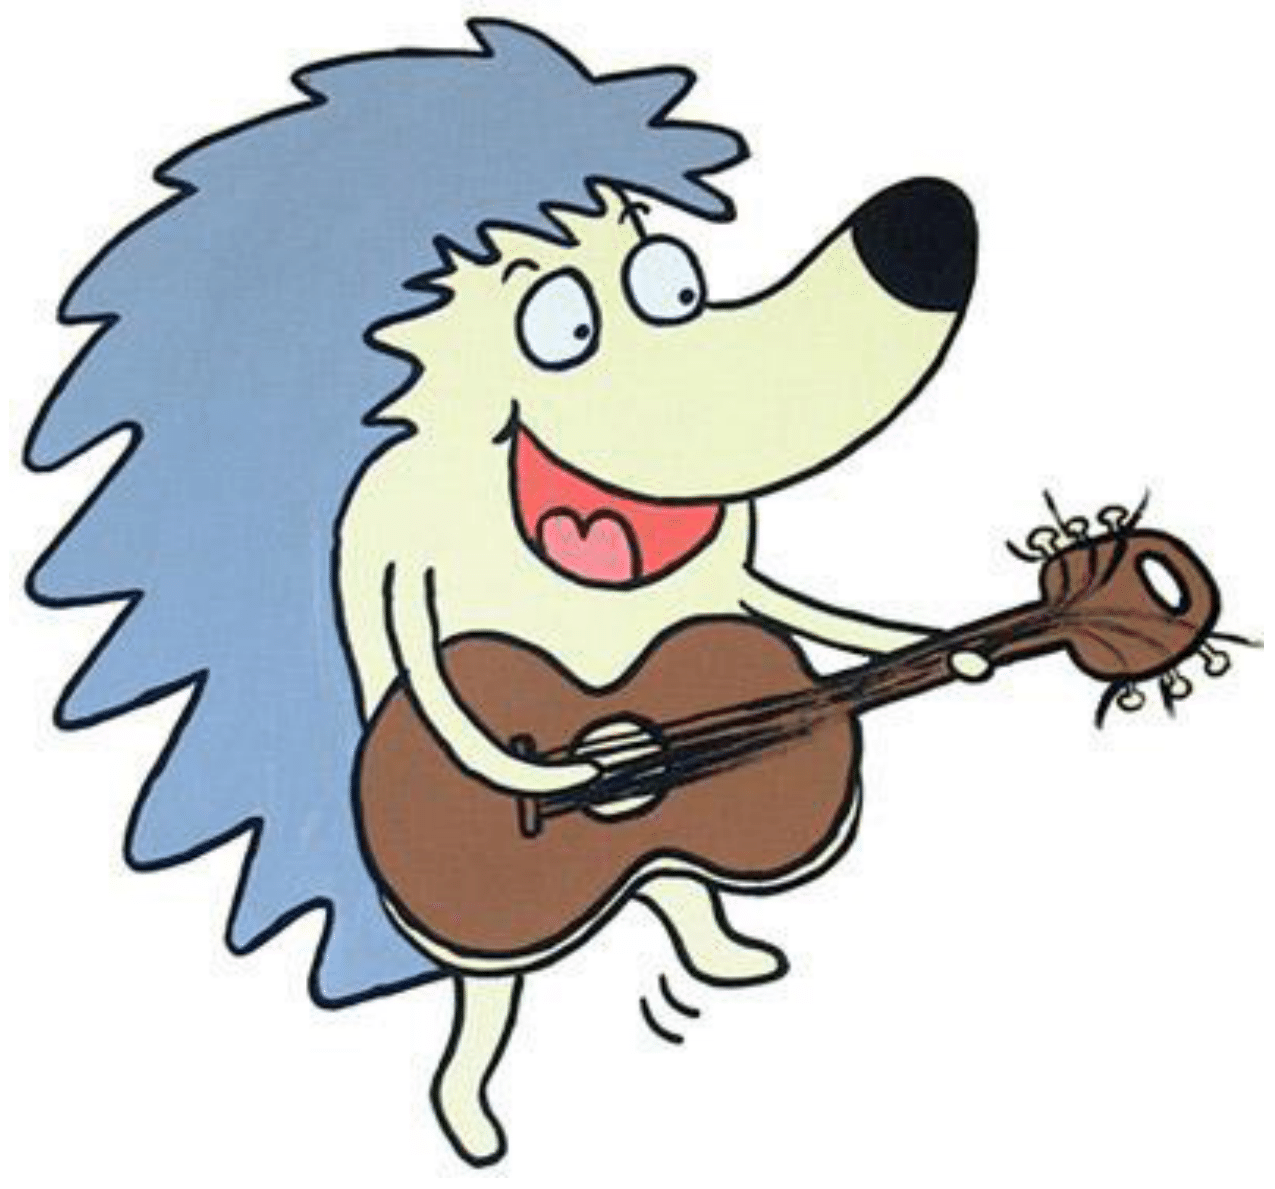
\includegraphics[scale=0.65]{jezek.png}\\
		\vspace{5em}
		{\fontsize{80}{90}\Fontskrivan\selectfont Zpěvník}
	\end{center}
	\end{figure}		
\end{titlepage}


% První strana
\pagenumbering{gobble}
\noindent Dílo je vytvořeno pod licencí Creative Commons (CC BY 4.0). Autorem je VasaM. Dílo smíte:
\begin{itemize}
	\item \textit{sdílet} -- rozmnožovat a distribuovat materiál prostřednictvím jakéhokoli média v jakémkoli formátu
	\item \textit{upravit} -- remixovat, změnit a vyjít z původního díla pro jakýkoliv účel, a to i komerční. 
\end{itemize} 
Za podmínky uvedení jeho původu, tedy je Vaší povinností uvést autorství, poskytnout s dílem odkaz na licenci a vyznačit Vámi provedené změny. Toho můžete docílit jakýmkoli rozumným způsobem, nicméně nikdy ne způsobem naznačujícím, že by poskytovatel licence schvaloval nebo podporoval Vás nebo Váš způsob užití díla. Poskytovatel licence nemůže odvolat tato oprávnění do té doby, dokud dodržujete licenční podmínky.\\
\\
\\
Zdrojové soubory k tomuto zpěvníku najdete na \url{https://github.com/VasaMM/zpevnik}. Vytvořené pdf tamtéž.\\
\\
\\
Ke zpěvníku byl vytvořen playlist pro službu Spotify \url{https://open.spotify.com/playlist/2eriz9vxG9uJzPwseSasVu?si=fcc7d09377ba4879}.\\
\\
\\
Tento soubor byl vytvořen \today.


% Obsah
\newpage
\tableofcontents
\thispagestyle{empty}
\pagenumbering{arabic}
\setcounter{page}{0}


% Písničky
\addContentSection{A}
\hlavicka[Vlasta Redl]{A te Rehradice}

\sloka{
\Emi A te Rehradice \D na pěkný ro\G vině,\\
\A teče tam vo\Hmi děnka \Emi dole \A po dě\D dině,\\
\Ami je pěk\Hmi ná, je \Emi čistá.
}

\sloka{
A po tej voděnce drobný rebe skáčó,\\
pověz ně má milá, proč tvý voči pláčó\\
tak smutně, žalostně.
}

\sloka{
Pláčou oni, pláčou šohajó pro tebe,\\
že sme sa dostali daleko vod sebe,\\
daleko vod sebe.
}

\sloka{
Co by neplakaly, když hlavěnka bolí\\
musijó zaplakat šohajovi kvóli\\
šohajovi kvóli.
}

\hlavicka{Anděl}{Karel Kryl}

\sloka{
\G Z rozmláce\Emi nýho kostela \G v krabici s \DSedm kusem mýdla\\
\G přinesl \Emi jsem si anděla, \G polámali \DSedm mu křídla,\\
\G díval se \Emi na mě oddaně, \G já měl jsem \DSedm trochu trému,\\
\G tak vtiskl \Emi jsem mu do dlaně \G lahvičku \DSedm od parfému.
}

\refren{
\G A proto, \Emi prosím, věř mi, \G chtěl jsem ho \DSedm žádat,\\
\G aby mi \Emi mezi dveřmi \G pomohl \DSedm hádat,\\
\G co mě čeká \EmiSiroky\DSedm a nemi\G ne,\\
\G co mě čeká \EmiSiroky\DSedm a nemi\G ne.
}

\sloka{
Pak hlídali jsme oblohu, pozorujíce ptáky,\\
debatujíce o Bohu a hraní na vojáky,\\
do tváře jsem mu neviděl, pokoušel se ji schovat,\\
to asi ptákům záviděl, že mohou poletovat.
}

\refren{}

\sloka{
Když novinky mi sděloval u okna do ložnice,\\
já křídla jsem mu ukoval z mosazný nábojnice,\\
a tak jsem pozbyl anděla, on oknem odletěl mi,\\
však přítel prý mi udělá novýho z mojí helmy.
}

\refren{}

\hlavicka{Až to se mnou sekne}{Jaromír Nohavica}
3/4 takt

\sloka{
\Ami Až obuju sirano \ESedm černe papirove \Ami boty,\quad\G\\
až i \C moja stara pocho\G pi, že nejdu do robo\C ty,\\
až \Dmi vyjde dluhy pruvod smutečnich hostu\\
na \Ami Slezsku Ostravu od Sykorova mostu,\\
\ESedm až to se mnu sekne, to bude \Ami pěkne,\\
\F pěkne, fajne a \Ami pěkne, \ESedm až to se mnu definitivně \Ami sekne.
}

\sloka{
Aby všeckym bylo jasne, že mě lidi měli radi,\\
ať je gulaš silny, baby smutne, muzika ať ladi,\\
bo jak sem nesnašel šledryjan ve vyrobě,\\
nebudu ho trpěť, ani co sem v hrobě,\\
to bude pěkne,\\
pěkne, fajne a pěkne, až to se mnu definitivně sekne.
}

\sloka{
S někerym to seka, že až neviš, co se robi,\\
jestli pomohla by deka nebo teplo mlade roby,\\
kdybych si moh vybrat, chtěl bych hned a honem,\\
ať to se mnu šlahne tajak se starym Magdonem,\\
to bude pěkne,\\
pěkne, fajne a pěkne, až to se mnu definitivně sekne.
}

\sloka{
Jedine, co nevim: jestli Startku nebo Spartu,\\
bo bych tam nahoře v nebi nerad trhal partu,\\
na každy pad s sebu beru bandasku s rumem,\\
bo rum nemuže uškodit, když pije se s rozumem,\\
to bude pěkne,\\
pěkne, fajne a pěkne, až to se mnu definitivně sekne.
}

\sloka{
Já vím, že, Bože, nejsi, ale kdybys třeba byl, tak\\
hoď mě na cimru, kde leži stary Lojza Miltag,\\
s Lojzu chodili sme do Orlove na zakladni školu,\\
farali sme dolu, tak už doklepem to spolu,\\
až to se mnu sekne,\\
pěkne, to bude pěkne, až to se mnu definitivně sekne.
}

\sloka{
Až obuju si rano černe papirove boty,\\
až i moja stara pochopi, že nejdu do roboty,\\
kdybych, co chtěl, dělal, všechno malo platne,\\
mohlo to byt horši, nebylo to špatne,\\
až to se mnu sekne,\\
k\F dybych, co chtěl, dělal, všechno malo platne,\\
m\Ami ohlo to byt horši, nebylo to špa\ESedm tne,\\
až to se mnu \dots\ na\F na na\dots \AmiSiroky\ESedmSiroky\AmiSiroky\FSiroky\AmiSiroky\ESedmSiroky\AmiSiroky
}

\addContentSection{B}
\hlavicka{Babička Mary}{Jan Werich, Jiří Voskovec}

\sloka{
\Ami Štěchovická \X laguna když dřímá \X v zadumaném stínu Kordy\X lér,\\
\Dmi pirát zkrva\Ami venou šerpu ždímá, \HSedm šerif si láduje revol\E ver.\\
\Ami Pikovická \X rýžoviště zlata \X čeří se v příboji Sáza\X vy,\\
\Dmi ale za to \Ami krčmářova chata \IDmi křepčí rykem \ESedm chlapské záb\IAmi avy.\\
\GSedm Když tu náhle, co se \C děje, \GSedm divný šelest houštím \C spěje,\\
\GSedm plch, skunk, \C vše utíká \IF po stráni \FisDim od Medn\IE íka.\\
\Ami Krčmář zhasne, \X kovbojové ztichnou, \X pirát zděšen tvář si zakry\X je,\\
\D rudé squaw se \Ami chvějí a pak vzdychnou:\\
\uv{\HSedm Blíží se k nám postrach préri\IE e}.\hspace{1em}\GSedm\hspace{1.5em}\I
}

\refrenX{1}{
\C Mary, \X babička \DSedm Mary, \X dva kolťá\GSedm ky za pasem,\\
\X nad hlavou \C točí lasem.\\
\X Stoletá \X Mary, \X babička \DSedm Mary, \X ta zkrotí \GSedm křepce hřebce,\\
\X ať chce či ne\IC chce.\ \ESedm\hspace{1.3em}\I
}

\sloka{
Žádné zuby, z jelenice sukně, ale za to tvrdé bicepsy,\\
Mary má vždy slivovici v putně, Toma Mixe strčí do kapsy.\\
Klika cvakla, v krčmě dveře letí a babička vchází do dveří,\\
\uv{Pintu ginu, lumpové prokletí!} bezzubou dásní zaláteří.\\
Vypiju to jen ve stoje, jdu do volebního boje,\\
zřím zas město drahý, jedu volit do Prahy.\\
Dopila a aby se neřeklo, putykáře změní v mrtvolu,\\
za zády má štěchovické peklo s šlajsnou svatojánských atolů.\\
}

\refrenX{2}{
Mary, babička Mary, pádluje bez námahy po proudu až do Prahy.\\
Stoletá Mary, babička Mary, jde do volebního boje za kovboje.\\
}
 
\sloka{
Ledva v Praze kotvu vyhodila, pro babičku nastal hrozný čas,\\
neboť hned každá strana tvrdila, že jí náleží babiččin hlas.\\
Malá stejně jako velká strana psala, že bude mít o hlas víc,\\
že ta druhá strana je nahraná, oni že maj hlas ze Štechovic.\\
Stoletý věk prý nevadí, na předáka je to mládí,\\
ze všech nejvíce, volala ji polnice.\\
Tak babičku, pro kterou vždy byla válka s lidojedy legrace,\\
tu babičku za pár dni zabila, volební agitace.\\
}


\refrenX{3}{
Mary, bojovná Mary, už nesedává v sedle, ve volbách byla vedle.\\
Stoletou Mary, babičku Mary, volbama zabitou vzal k sobě Manitou.\\
}
 
\hlavicka{Batalion}{Spirituál kvintet}

3/4 takt

\sloka{
\Ami Víno \C máš a \G marky\Ami tánku, \X dlouhá \C noc se \G prohý\Ami ří.\\
Víno máš a chvilku spánku, díky, díky verbíři.
}

\sloka{
\Ami Dříve, než se roze\X dní, kapitán \IC k osedlání \G rozkaz \IAmi dá\hspace{1.7em}\Emi vá,\quad\I\\
\Ami ostruhami do sla\IX bin   ko\G ně \IAmi po\hspace{1.7em}\Emi há\hspace{1.2em}\IAmi ní.\\
Tam na straně polední čekají ženy, zlaťáky a sláva,\\
do výstřelu karabin zvon už vyzvání.
}

\refren{
\Ami Víno na ku\C ráž a \G pomilovat marky\Ami tánku,\\
\Ami zítra do Bur\IC gund batalion\IAmi\ za\hspace{1.5em}\Emi mí\hspace{1.3em}\IAmi ří.\\
Víno na kuráž a k ránu dvě hodinky spánku,\\
díky, díky vám královští verbíři.
}

\sloka{
Rozprášen je batalion, poslední vojáci se k zemi hroutí,\\
na polštáři z kopretin budou věčně spát.\\
Neplač sladká Marion, verbíři nové chlapce přivedou ti,\\
za královský hermelín padne každý rád.
}

\refren{}

\slokaOpakovani{1.}{}
 \hlavicka[bratři Ryvolové]{Bedna od whisky}

\sloka{
\Ami Dneska už mě \C fóry ňák \Ami nejdou přes \E pysky \\
\Ami Stojím s dlouhou \C kravatou na \IAmi bedně \E vod wh\IAmi isky. \\
Stojím s dlouhým \C vobojkem jak \Ami stájovej \E pinč. \\
\Ami Tu kravatu \C co nosím mi \IAmi navlík \E soudce\IAmi\ Linč.\quad\X
}

\refren{
\A Tak \X kopni do tý \D bedny ať \E panstvo neče\A ká \\
jsou \X dlouhý schody do \D nebe a \E štreka dale\A ká. \\
Do \X nebeskýho \D báru já \E sucho v krku \A mám. \\
Tak \X kopni do tý \D bedny ať \E na cestu se \A dám.\ hspace{1em}\XSiroky\XSiroky\XSiroky
}

\sloka{
Mít tak všechny bedny od whisky vypitý. \\
Postavil bych malej dům na louce ukrytý. \\
Postavil bych malej dům a z okna koukal ven \\
a chlastal bych tam s Billem a chlastal by tam Ben.
}

\refren{}

\sloka{
Kdyby si se hochu jen pořád nechtěl rvát. \\
Nemusel jsi dneska na týhle bedně stát. \\
Moh si někde v suchu tu svoji whisky pít\\
nemusel si hochu na krku laso mít.
}

\refren{}

\sloka{
Když jsem štípnul koně a ujel jen pár mil\\
nechtěl běžet dokavád se whisky nenapil\\
zatracená smůla zlá a zatracenej pech\\
když kůň cucá whisku jak u potoka mech.
}

\refren{}

\sloka{
Až kopneš do tý bedny, jak se to dělává \\
do krku ti zůstane jen dírka mrňavá. \\
Jenom dírka mrňavá a k smrti jenom krok. \\
mám to smutnej konec - a whisky ani lok
}

\refren{Tak kopni do tý bedny ať panstvo nečeká \\
jsou dlouhý schody do nebe a štreka daleká. \\
Do nebeskýho báru já sucho v krku mám\\
tak kopni do tý bedny!}
\zvyraznit
\takt{6}{8}
\hlavicka[Pavel Dydovič]{Bláznova ukolébavka}

\sloka{
\G Máš má ovečko \D dávno spát, i \C píseň ptáků \G končí,\\
\X kvůli nám přestal \D vítr vát, jen \C můra zírá \G zvenčí\\
Já \D znám její zášť tak \C vyhledej skrýš,\\
zas \D má bílej plášť a \IC v okně je \D mříž\I .
}

\refren{
\G Máš má ovečko \D dávno spát\\
a \C můžeš hřát ty mně \A můžeš hřát\\
Vždyť \G přijdou se \C ptát,\\
zítra zas \G přijdou se \C ptát\\
jestli ty v \G mých předsta\C vách už \G mizíš.
}

\sloka{
Máš má ovečko dávno spát, dnes máme půlnoc temnou.\\
Ráno budou nám bláznům lát, že ráda snídáš se mnou.\\
Proč měl bych jim lhát že jsem tady sám,\\
když tebe tu mám když tebe mám rád.
}
\hlavicka[Greenhorns]{Blues Folsomské věznice}

\sloka{
\G Můj \X děda bejval \X blázen, te\X xaskej Ahas\X ver,\\
a \X na půdě nám \X po něm zůstal \GSedm ošoupanej \X kvér.\\
Ten \C kvér obdi\X vovali všich\X ni kámoši \X z oko\G lí\\
a \D máma mi ří\X kala: „\X Nehraj si s tou \DSedm pisto\G lí!“
}

\sloka{
Jenže i já byl blázen tak zralej pro malér\\
a ze zdi jsem sundával tenhle ten dědečkův kvér.\\
Pak s kapsou vyboulenou chtěl jsem bejt chlap \uv{All right}\\
a s holkou vykutálenou hrál jsem si na Boonie and Clyde.
}

\sloka{
Ale udělat banku, to není žádnej žert,\\
sotva jsem do ní vlítnul hned zas vylít' jsem jak čert.\\
Místo jako kočka já utíkám jak slon,\\
takže za chvíli mě veze policejní anton.
}

\sloka{
Teď okno mřížovaný mně říká, že je šlus,\\
proto tu ve věznici zpívám tohle Folso blues.\\
Pravdu měla máma, radila: Nechoď s tou holkou!\\
a taky mně říkala: Nehraj si s tou pistolkou!
}

\hlavicka{Blues na cestu poslední}{Semafor}

\sloka{
\D Černej nebožtíku, \GSedm máš to ale kliku,\\
\D za chvíli do temný hlíny \DSedm budeš zakopán,\\
\GSedm Černej nebožtíku, \X máš to ale kliku,\\
\D za chvíli do temný hlíny \X budeš zakopán,\\
\ASedm nás jsi nechal v bídě, \GSedm sám se vezeš jako \D pán.
\FisDim\hspace{4em}\Fdim\hspace{3.5em}\D\hspace{2em}\DisDim\hspace{4.2em}\ASedm
} 

\sloka{
Jen kopyta koní hrany tobě zvoní,\\
málo lidí dnes pro tebe slzy polyká,\\
je to smutnej funus, chybí ti tu muzika.
}

\sloka{
Kam ti pozůstalí, kam ti vlastně dali\\
věnce, kytky, pentle, svíce, marně se ptám,\\
proč je rakev holá, to ty asi nevíš sám.
}

\sloka{
Černej nebožtíku, když nemáš na muziku,\\
poslechni mou radu trochu nevšední,\\
zazpívej si sám blues na cestu poslední.
}

\hlavicka[Petr Kalandra]{Břímě}

\sloka{
\G Včera mě spolkl \Hmi Nazareth, aby \C dnes vypliv ostatky \G mý\\
celou noc hledám místo kam složit vlasy šedivý\\
hej pane nechcete mi říct, kde tu můžu složit hlavu svou\\
né řekl a hned zmizel tam za tou velkou bílou budovou.
}

\refren{
\G Sundej \Hmi z něj to \C břímě \G a nechtěj \Hmi za to \C nic\\
\G dědek ať \Hmi už se \C nedře, hej, hej, héééj \\
nandej mi ho na zá\G da.\HmiSiroky\CSiroky\GSiroky\DSiroky\EmiSiroky\DSiroky\CSiroky
}

\sloka{
Přes rameno ranec svůj, jak rád bych nějaký místo měl\\
kam bych se v klidu schoval a na všechno bych zapomněl\\
v tom vidím Carmen s Ghiou jak po ulici proti jdou\\
Carmen že nemá čas, že si spolu rychle užijou.
}

\refren{
Sundej z nich to břímě a nechtěj za to nic holky ať už se nedřou\dots
}

\sloka{
Když přijdeš k paní Mósrové, tak tam není co bys řek\\
připadáš si jak v automatu ve frontě na párek\\
povídá: \uv{Mladej kmete, a což takhle třeba Nathalii?}\\
už není právě nejmladší a tak zůstaň dneska večer s ní.
}

\refren{
Sundej z ní to břímě a nechtěj za to nic holka ať už se nedře\dots
}

\sloka{
Postarší právník mě nakop a to rovnou do koulí\\
povídá já ti cestu ukážu ale musíš s mým psem ven\\
povídám moment soudče já jsem taky Homo sapiens\\
Abych si trochu ulehčil tu ránu jsem mu navrátil.
}

\refren{
Sundej z něj to břímě a nechtěj za to nic dědek ať už se nedře\dots
}

\sloka{
Na dělový kouli z roku 1835 se vezu někam dolů,\\
je načase mi závidět.\\
Tak letím mezi vás, pozdravuje vás tamten svět\\
že prej se nemusíte vracet, je načase mi závidět
}

\refren{
Sundej ze mě to břímě a nechtěj za to nic ať už se nikdy nedřu\dots nandej si ho na záda.
}

\hlavicka[Michal Tučný]{Buráky}

\sloka{
Když \D Sever válčí s Jihem \IG a zem jde do vá\D lky, na\I\\
\X polích místo bavlny te\IE ď rostou bodláky.\ASedm Ve\ \I\\
\D stínu u silnice vidí\IG m z Jihu vojá\D ky, jak\I\\
\X válejí se líně \IASedm a louskaj burá\D ky.\ \I
}

\refren{
Hej \D hou, hej hou, na\IG č chodit do vá\D lky, je\I\\
\X lepší doma sedět \IE a louskat bur\ASedm áky. Hej\I\\
\D hou, hej hou, na\IG č chodit do vá\D lky, je\I\\
\X lepší dom\IASedm a sedět a louskat burá\D ky.\I
}

\sloka{
Plukovník je v sedle, volá: \uv{Yankeeové jdou!},\\
ale mužstvo v trávě leží, prej dál už nemohou,\\
plukovník se otočí a koukne do dálky,\\
tam jeho slavná armáda teď louská buráky.
}

\refren{}

\sloka{
Až tahle válka skončí a my zas budem žít,\\
svý milenky a ženy pak půjdem políbit,\\
Když se zeptaj: \uv{Hrdino, cos dělal za války?}\\
\uv{Já flákal jsem se s kvérem a louskal buráky.}
}

\refren{}
\addContentSection{C}
\hlavicka{Cesta}{Kryštof}

\sloka{
Tou \C cestou,
tím směrem prý, bych se dávno měl \G dát.\\
Když \Ami sněží, jde to stěží, ale sněhy pak tají.\\
Kus \F něhy ti za nehty \G slíbí a dají.  \\
Víc síly se prát, na dně víc dávat než brát.\\
A i když se vleče a je schůdná jen v kleče,\\
donutí přestat se zbytečně ptát.
}

\refren{
Jestli se \C blížím k cíli,\\
kolik \G zbývá víry, kam \Ami zvou\\
svodidla, co po tmě mi \F lžou?\ \G\\
Zda couvám zpátky\\
a plýtvám řádky, co řvou,\\
že už mi doma neotevřou .
}

\sloka{
Nebo jít s proudem,\\
na lusknutí prstu se začít hned smát.\\
Mít svůj chodník slávy a před sebou davy\\
a přes zkroucená záda být součástí stáda.\\
Ale zpívat a hrát, kotníky líbat, a stát,\\
na křídlech všech slavíků, a vlastně už ze zvyku,\\
přestat se zbytečně ptát.
}

\refren{}
\refren{}

\hlavicka{Čůrej!}{Kašpárek v rohlíku}

\slokaBezCisla{\DSiroky\GSiroky\DSiroky\hspace{1em}\DSiroky\GSiroky\DSiroky}

\sloka{
Čůrej sem a čůrej tam,\DSiroky\GSiroky\DSiroky\\
čůrej jako velkej pán.\DSiroky\GSiroky\DSiroky\\
Ve stoje i za běhu,\GSiroky\FSiroky\GSiroky\\
žlutý srdce do sněhu.\DSiroky\GSiroky\DSiroky\\
Každej se rád vyčůrá,\ASiroky\ASedmSiroky\\
zadara i za bůra.\DSiroky\GSiroky\DSiroky
}

\sloka{
Čůrej sem, sem, sem,\\
čůrej dovnitř, čůrej ven,\\
řekni mi kam čůrat mám,\\
já se ti tam vyčůrám.\\
Ať jsi s partou nebo sám,\\
čůrej sem a čůrej tam.
}

\refren{
Ať seš velkej nebo \D malej,\GSiroky\DSiroky\\
do sklenice vodu \D nalej,\GSiroky\DSiroky\\
ten kdo hodně vody \G lemtá,\FSiroky\GSiroky\\
přečůrá i \D prezidenta.\GSiroky\DSiroky\\
A když nevíš kudy \D kam,\GSiroky\DSiroky\ASiroky
}

\sloka{
3. Čůrej doma, čůrej v metru, (hlavně rychle ještě dneska)\\
jen nečůrej proti větru! (skvělej výkon všichi tleskaj)\\
Malí ještě nevinný, (můžou čůrat do plíny)\\
maj to pěkně s rámusem. \\
Ať jsi s partou nebo sám, (holky se maj můžou sedět)\\
čůrej sem a čůrej tam. (holky se maj můžou sedět)
}

\refren{}

\sloka{
Čůraj Češi, čůraj Němci,\\
hrozně tupí vytlemenci,\\
někdy kýbl, někdy deci.\\
Na dnešek mám dobrej plán.\\
Čůrat sem a čůrat tam\A .
}

\addContentSection{D}
\hlavicka{Divoké koně}{J. Nohavica}
 
\sloka{
\repetice{\Ami Já viděl \IDmi divoké \Ami koně,\IC\ běželi \Dmi soumrakem\IAmi ,}
\IDmi vzduch \Ami těžký\I\ \IDmi byl a divně \Ami voněl \IDmi tabá\quad\F kem,\\
\IDmi vzduch \Ami těžký\I\ \IDmi byl a divně \Ami voněl \ESedm tabá\IAmi kem.
}

\sloka{
\repetice{Běželi, běželi bez uzdy a sedla krajinou řek a hor,}
\repetice{sper to čert, jaká touha je to vedla za obzor?}
}

\sloka{
\repetice{Snad vesmír nad vesmírem, snad lístek na věčnost,}
\repetice{naše touho, ještě neumírej, sil máme dost.}
}

\sloka{
\repetice{V nozdrách sládne zápach klisen na břehu jezera,}
\repetice{milování je divoká píseň večera.}
}

\sloka{
\repetice{Stébla trávy sklání hlavu, staví se do šiku,}
\repetice{král s dvořany přijíždí na popravu zbojníků.}
}

\sloka{
\repetice{Chtěl bych jak divoký kůň běžet, běžet, nemyslet na návrat,}
\repetice{s koňskými handlíři vyrazit dveře, to bych rád.}
Já viděl divoké koně\dots
}

\zvyraznit
\hlavicka[Chinaski]{Dobrák od kosti}

\sloka{
\D Má milá \A jak ti je, tak \G jak ti je?\ \X\\
\D Jsem ten, kdo \A jednou tvý \G tělo zakryje.\ \CaddDevet\\
Jsem ten, kdo tě jednou oddělá.\\
Potkala's zkrátka koho's neměla.
}

\sloka{
\DSiroky\ASiroky\GSiroky\GSiroky\\
Jsi budoucí krev v mojí posteli.\\
Jsem ten, kdo tě jednou jistojistě zastřelí.\\
Jsem ten kdo ty tvoje krásný oči jednou zatlačí.\\
Jsi moje všechno a mě to nestačí.
}

\refren{
\D Je to vážně silná \X káva, \A pláč a nebo \X vztek \G nic už s tím \X nenaděláš,\\
\D nech mě jenom \X hádat, \A jak jsi hebká na \X dotek \G krásná a \X nedospělá.
}

\sloka{
Víš, všechno má aspoň malý kaz,\\
jsem ten, kdo ti jednou zlomí vaz.\\
Má milá vždyť mě znáš jsem dobrák od kosti,\\
a ty jsi ta co mi to jednou všechno odpustí.
}

\sloka{
\D Sejde z očí \X sejde z mysli,\\
\A jenom blázen věří \X na nesmysly,\\
\G láska je čaroděj \X a ticho prý léčí,\\
\X ale zákon hovoří \X jasnou řečí.
}

\refren{}

\slokaBezCisla{
\D Má milá \A jak ti je, tak \G jak ti je?\ \X\\
\D Jsem ten, kdo \A jednou tvý \G tělo zakryje.\ \CaddDevet
}

\vspace{-25em}
\noindent\hspace*{27em}\hmat[]{p3,p2,n,n,p3,p3}{\akordhmat{G}}\\
\\\\
\noindent\hspace*{27em}\hmatCaddDevet


\hlavicka{Dokud se zpívá}{Jaromír Nohavica}

3/4 takt

\sloka{
\C Z Těšína \Emi vyjíždí \DmiSedm vlaky co \F čtvrthodi\C nu,\quad\EmiSiroky\DmiSedmSiroky\GSedmSiroky\\
\C včera jsem \Emi nespal a \DmiSedm ani dnes \F nespoči\C nu,\quad\EmiSiroky\DmiSedmSiroky\GSedmSiroky\\\F 
\F svatý Med\G ard, můj pa\C tron, ťuká \IC si na \Ami če\hspace{1.3em}\IG lo,\quad\G\\
\F ale dokud se \G zpívá, \F ještě se \G neumře\C lo, \Emi hó\hspace{1.2em}\DmiSedm hó.\hspace{1.5em}\GSedm
}

\sloka{
Ve stánku koupím si housku a slané tyčky,\\
srdce mám pro lásku a hlavu pro písničky,\\
ze školy dobře vím, co by se dělat mělo,\\
ale dokud se zpívá, ještě se neumřelo, hóhó.
}

\sloka{
Do alba jízdenek lepím si další jednu,\\
vyjel jsem před chvílí, konec je v nedohlednu,\\
za oknem míhá se život jak leporelo,\\
ale dokud se zpívá, ještě se neumřelo, hóhó.
}

\sloka{
Stokrát jsem prohloupil a stokrát platil draze,\\
houpe to, houpe to na housenkové dráze,\\
i kdyby supi se slítali na mé tělo,\\
tak dokud se zpívá, ještě se neumřelo.
}

\sloka{
Z Těšína vyjíždí vlaky až na kraj světa,\\
zvedl jsem telefon a ptám se: \uv{Lidi, jste tam?}\\
A z veliké dálky do uší mi zaznělo,\\
že dokud se zpívá, ještě se neumřelo.\\
Že dokud se zpívá ještě se neumřelo.
}


\hlavicka{Ďábel a syn}{Kabát}

\sloka{
\Dmi Sedím a koukám jak \C zvrácenej podzim\\
\Ami stromům svlíká jejich \G šat\\
\Dmi poslouchám ptáky a \C jenom tak kouřím\\ 
\Ami malinko chce se mi \G spát\\\\ 
Padá mi hlava pak cejtím jak někdo\\ 
lehce mě za ruku vzal\\
blázen či voják jak maškara divná\\ 
tam \Ami stál já pozval ho \Dmi dál\
}


\sloka{
Měl špinavej kabát a v ruce flétnu\\
oči jak z mrtvejch by vstal\\
na botách bahno snad celýho světa\\ 
a tuhletu píseň mi hrál\\\\
Tu píseň co zpívám a vůbec vám nevím\\ 
kde na ni akordy vzal\\
jak sem tam seděl a koukal a kouřil\\ 
to já teprv ji psal 
}

\sloka{
Povídá hochu vracim se z flámu\\ 
hráli jsme karty se zdá\\
partii pokera o budoucí vládu\\
dík bohu vyhrál jsem já\\\\
Já měl z pekla štěstí a nebo pár trumfů\\ 
v rukávu podvod - já vím\\
chcete mě soudit tak dejte mě na kříž\\ 
jsem váš ďábel a syn
}

\sloka{
Pak pomalu mluvil a ničil mě silou\\
co od věků v sobě už má\\
drtil mě pravdou a pouštěl mi žilou\\
na závěr jen povídá\\\\
Bůh stvořil lásku a žal taky bolest\\
a já jenom ubohej chtíč\\
fandím vám lidem nevím proč nemáš\\
mě rád já poslal ho pryč
}

\sloka{
Sedím a koukám jak zvrácenej podzim\\ 
stromům svlíká jejich šat\\
poslouchám ptáky a jenom tak kouřim\\
a malinko chce se mi spát\\\\
Padá mi hlava pak cejtim jak někdo\\ 
lehce mě za ruku vzal\\
blázen či voják jak maškara divná\\ 
tam stál tak pozvem ho dál
}

\addContentSection{F}
\hlavicka{Frankey Dlouhán}{Nedvědi}

\sloka{
Kolik je \C smutného když \F mraky černé \C jdou\\
\X lidem nad hlavou \GSiroky\F smutnou dála\C vou\\
\X\quad já slyšel \X příběh, který \F velkou pravdu \C měl\\
\X za čas odletěl, \GSedmSiroky\F každý zapo\C mněl
}

\refren{
\C Měl kapsu \GSedm prázdnou Frankey \X Dlouhán \\
po státech \F toulal se jen \C sám\\
a že byl \F veselej tak \C každej měl ho \GSedm rád\\
\GSedm  tam ruce \F k dílu mlčky \X přiloží\\
a \C zase jede \Ami dál a \F každej, \\
kdo s ním \GSedm chvilku byl, tak \IF dlouho \GSedm se pak smál\IC .\hspace{2em}\X
}

\sloka{
Tam, kde byl pláč, tam Frankey hezkou píseň měl \\
slzy neměl rád, chtěl se jenom smát\\
a když pak večer ranče tiše usínaj\\
Frankův zpěv jde dál nocí s písní dál.
}

\refren{}

\sloka{
Tak Frankyho vám jednou našli přestal žít, \\
jeho srdce spí tiše smutně spí\\
Bůhví a za co tenhle smíšek konec měl \\
farář píseň pěl umíráček zněl.
}

\refren{}

\addContentSection{G}
\takt{2}{4}
\hlavicka[Čechomor]{Gorale}

\sloka{
\D Za lasami za \G gorami \A za dolina\D mi\\
\D pobiłi się \G dwaj gorale \A ciupaga\D mi.
}

\refren{
\repetice{ Ej gora\G le, \A nie bijta \D się\\
\X ma góralka \G dwa warkocze\\
\A podzielita \D się.}
}

\sloka{
Za lasami za gorami§\dots\\
ma goralka dwoje oczu podzielita się.
}

\sloka{
Za lasami za gorami\dots\\
ma goralka wielke serce podzielita się.
}

\sloka{
Za lasami za gorami\dots\\
ma goralka z przodu z tyłu podzielita się.
}

\addContentSection{H}
\hlavicka{Hlídač krav}{Jaromír Nohavica}

\vspace*{1em}
\DSiroky\DSiroky\DSiroky\DSiroky
\vspace{-1em}
\repetice{\D Pam pam pa dam \X pam pa dam pam \X pam pam pa dam \X pam pa dam pam\\
\G Pam pa da da dam \ASedm pa da da dam.\DSiroky\X}

\sloka{
\D Když jsem byl malý, \X říkali mi naši:\\
\X Dobře se uč a \X jez chytrou kaši,\\
\G až jednou vyrosteš, \ASedm budeš doktorem práv. \DSiroky\X\\
Takový doktor sedí pěkně v suchu,\\
bere velký peníze a škrábe se v uchu,\\
já jim ale na to řek: chci být hlídačem krav.
}

\refren{
Já chci mít čapku s bambulí nahoře,\\
jíst kaštany a mýt se v lavoře,\\
od rána po celý den zpívat si jen.\\
Zpívat si: pam \dots\DSiroky\DSiroky\DSiroky\GSiroky\ASedmSiroky\DSiroky\DSiroky
}

\sloka{
K vánocům mi kupovali hromady knih,\\
co jsem ale vědět chtěl, to nenašel jsem v nich,\\
nikde jsem se nedozvěděl, jak se hlídají krávy.\\
Ptal jsem se starších a ptal jsem se všech,\\
každý na mě koukal jako na pytel blech,\\
každý se mě opatrně tázal na moje zdraví.
}

\refren{}

\sloka{
Dnes už jsem starší a vím, co vím,\\
mnohé věci nemůžu a mnohé smím,\\
a když je mi velmi smutno, sednu do mokré trávy.\\
S nohama křížem a s rukama za hlavou\\
koukám nahoru na oblohu modravou,\\
kde se mezi mraky honí moje strakaté krávy.
}

\refren{}
\zvyraznit
\hlavicka[Žalman]{Ho ho Watanay}

\sloka{
\D Spinkej můj \X maličký, \C máš v očích \D hvězdičky,\\
\X dám ti je \C do vlasů tak \G usínej tak \D usínej.
}

\refren{
\D Ho ho \X Watanay \C ho ho \D Watanay\\
\X ho ho \C Watanay Kio\G kena Kio\D kena.
}

\sloka{
Sladkou vůňi nese ti noční motýl z perleti,\\
vánek ho kolíbá, už usíná, už usíná.
}

\refren{}

\sloka{
V lukách to zavoní, rád jezdíš na koni,\\
má barvu havraní, jak uhání jak uhání.
}

\refren{}

\sloka{
V dlani motýl usíná, hvězdička už zhasíná,\\
vánek co ji k tobě nes, až do léta ti odlétá.
}

\refren{}
\takt{3}{4}
\hlavicka[Čechomor]{Hruška}

\sloka{
Sto\D jí hruška v ši\A rém po\D li, vr\X šek se jí \G zele\A ná.\\
\repetice{\D\ \ Pod \G ní se \A pase \D kůň vra\X ný, pa\X se ho \A má mi\D lá.}
}

\sloka{
Proč má milá dnes pasete, z večera do rána?\\
\repetice{Kam můj milý pojedete, já pojedu s váma.}
}

\sloka{
O já pojedu daleko, přes vody hluboké.\\
\repetice{Kéž bych byl nikdy nepoznal, Anny černooké.}
}
\hlavicka{Hudsonský šífy}{Wabi Daněk}

\sloka{
\akord{4$\times$A\akordMi}\hspace{1.5em}Ten kdo \X nezná hukot vody\\
lopat\C kama vířený jako \G já, jako \C já.\\
Kdo Hud\Ami sonský slapy nezná\\
sírou \G pekla sířený, ať se na \Ami hudsonský\\
\G šífy najmout \Ami dá,\quad\G jo ho \Ami ho.\\
\\
Ten kdo nepřekládal uhlí, šíf když na\\
mělčinu vjel, málo zná, málo zná.\\
Ten kdo neměl tělo ztuhlý\\
až se nočním chladem chvěl,\\
ať se na hudsonský šífy najmout dá, jo ho ho.
}

\refren{
Tak \F ahoj, páru tam \Ami hoď,\\
ať \G do pekla se dřívě dohra\Ami bem.\\
\G Jo ho \Ami ho,\quad\G jo ho \Ami ho.
}

\sloka{
Ten kdo nezná noční zpěvy\\
zarostenejch lodníků, jako já, jako já.\\
Ten kdo cejtí se bejt chlapem, umí dělat rotyku,\\
ať se na hudsonský šífy najmout dá, jo ho ho.\\
Ten kdo má na bradě mlíko,\\
kdo se rumem nevopil, málo zná, málo zná.\\
Kdo necejtil hrůzu z vody, kde se málem utopil\\
ať se na hudsonský šífy najmout dá, jo ho ho.
}

\refren{}

\sloka{
Kdo má roztrhaný boty,\\
kdo má pořád jenom hlad, jako já, jako já.\\
Kdo chce celý noci čuchat\\
pekelního ohně smrad, ať se na hudsonský šífy\\
najmout dá, jo ho ho. Kdo chce zhebnout \\
třeba zejtra, komu je to všechno fuk,\\
kdo je sám, jako já,\\
Kdo má srdce v správným místě,\\
kdo je prostě prima kluk,\\
ať se na hudsonský šífy najmout dá, jo ho ho.
}

\refren{}

\hlavicka{Husličky}{Vlasta Redl}

\sloka{
\repetice{\A Čí že ste, husličky, \D či-\A e, \Hmi kdo vás tu \FisMi zane\hspace{1em}\E chal}
\HmiSedm na trávě \E pová\A lané\D,\hspace{1em}\Hmi na trávě \E pov\A ála\D né\Hmi\ u paty \FisMi ořech\E a?\hspace{.7em}\HmiSiroky\FisMiSiroky\ESiroky
}

\sloka{
\repetice{A kdože tu trávu tak zválal, aj modré fialy,}
že ste, husličky, samé, že ste, husličky, samé na světě zostaly?
}

\sloka{
\repetice{A který tu muzikant usnul a co sa mu přišlo zdát,}
co sa mu enem zdálo, bože co sa mu enem zdálo,\\
že už vjec nechtěl hrát?
}

\sloka{
\repetice{Zahrajte, husličky, samy, zahrajte zvesela,}
až sa tá bude trápit, až sa tá bude trápit, která ho nechtěla.
}
\hlavickaStar{Hvězdář}{UDG}

\sloka{
Ztrácíš se \D před očima, rosteš jen \A ve vlastním stínu.\\
Každá \Emi další vina, odkrývá \CmajSedmG mojí vinu.\\
Ztrácíš se \D před očima, rosteš jen \A ve vlastním stínu.\\
Každá \Emi další vina, odkrývá \CmajSedmG mojí vinu. \emph{[Ve vínu}
}

\sloka{
\repetice{Ve vínu \D dávno nic nehled\A ám. \EmiSiroky\CmajSedmGSiroky}
}

\refren{
\repetice{Jak luna mizí s nocí v bělostných šatech pro nemocné,\\
prosit je zvláštní pocit, jen ať je den noc ne.}
}

\sloka{
\repetice{Od proseb dávno nic nečekám.}
}

\sloka{
Na chodbách v bludných kruzích zářivka vyhasíná,\\
já ti do infuzí chci přilít trochu vína.\\
Na nebi jiných sluncí, jak se tam asi cítíš,\\
s nebeskou interpunkcí, jiným tulákům svítíš.
}

\slokaOpakovani{2.}{}

\refren{}

\sloka{
(3x)\repetice{\D Obzor než klesne níž, \A je ráno a ty spíš.\\
\Emi Od vlků odraná \CmajSedmG hvězdáře Giordána.}
Odpouštíš
}

\vspace{-5em}
\begin{center}
~~\hspace{25em}~~\hmatCmajSedmD~~
\end{center}
\addContentSection{J}
\zvyraznit
\hlavicka[Fešáci]{Jaro}

\sloka{
\Ami My čekali \C jaro, a \G zatím přišel \Ami mráz,\quad\X\\
tak strašlivou zimu nepoznal nikdo z nás,\\
z těžkých černých mraků se stále sypal sníh\\
a vánice sílí v poryvech ledových.\\
\C Z chýší dřevo \X mizí a \G mouka ubý\X vá,\\
\Dmi do sýpek se \X raději už \G nikdo nedí\X vá,\\
\C zvěř z okolních \X lesů nám \G stála u dve\X ří\\
\Dmi a hladoví \X ptáci při\G létli za zvě\X ří, a stále \Ami blíž.\quad\X
}

\sloka{
Tak jednoho dne večer, to už jsem skoro spal,\\
když vystrašenej soused na okno zaklepal:\\
\uv{Můj chlapec doma leží, v horečkách vyvádí,\\
já do města bych zajel, doktor snad poradí.}\\
Půjčil jsem mu koně, a když sedlo zapínal,\\
dříve, než se rozjel, jsem ho ještě varoval:\\
\uv{Nejezdi naší zkratkou, je tam velkej sráz\\
a v týhletý bouři tam snadno zlámeš vaz, tak neriskuj!}
}

\sloka{
Na to smutné ráno dnes nerad vzpomínám,\\
na tu hroznou chvíli, když kůň se vrátil sám,\\
trvalo to dlouho, než se vítr utišil,\\
na sněhové pláně si každý pospíšil.\\
Jeli jsme tou zkratkou až k místu, které znám,\\
kterým bych v té noci nejel ani sám,\\
a pak ho někdo spatřil, jak leží pod srázem,\\
krev nám tuhla v žilách nad tím obrazem, já klobouk sňal.
}

\sloka{
\Ami Někdy ten, kdo \C spěchá, se \G domů nevra\Ami cí\dots
}
\hlavicka[Olympic]{Jasná zpráva}

\slokaBezCisla{
\CSiroky\AmiSiroky\FSiroky\GSiroky\DmiSiroky\FSiroky\akord{($\mathbf{2\times}$)}
}

\sloka{
\G Skončili jsme jasná zpráva,\\
\IEmi proč o tebe \C zakopávám\ID\ dál,\\
\IAmi projít bytem \C já abych s\IG e bál.\\
\\
Dík tobě se vidím zvenčí,\\
připadám si starší menší sám,\\
kam se kouknu, kousek tebe mám.
}

\refren{
\IEmi Pěnu s vůni \G jablečnou,\IEmi\ vyvanulý \Hmi sprej,\I\\
\IEmi telefon, cos \G ustřihla mu\ID\ šňůru,\\
\IEmi knížku krásně \G zbytečnou,\IEmi\ co má lživý \Hmi děj,\hspace{.7em}\I\\
\IEmi píše se v ní, \G jak se lítá\ID\ vzhůru,\\
lítá \Ami vzhůru, ve dvou \D vzhůru.
}

\sloka{
Odešla's mi před úsvitem,\\
mám snad bloudit vlastním bytem sám,\\
kam se kouknu, kousek tebe mám.
}

\refren{}

\sloka{
Skončili jsme jasná zpráva,\\
není komu z okna mávat víc,\\
jasná zpráva, rub, co nemá líc.
}

\hlavicka{Jdem zpátky do lesů}{Žalman}

\sloka{
\AmiSedm Sedím na kolejích, \DSedm které nikam neve\G dou,\hspace{1em}\X\\
\AmiSedm koukám na kopretinu, jak \DSedm miluje se s lebe\G dou.\hspace{1em}\X\\
\AmiSedm Mraky vzali slunce, \DSedm zase pod svou ochra\G nu,\hspace{1em}\Emi\\
\AmiSedm jen ty nejdeš holka zlatá, \DSedm kdypak já tě dosta\G nu.\hspace{1em}\DSedm
}

\refren{
\G Z ráje, \X my vyhnaní \Emi z ráje,\\
\X kde není už \AmiSedm místa, \CSedmSiroky prej něco se \G chystá.\hspace{1em}\DSedm\\
\G Z ráje, \X nablýskaných \Emi plesů,\\
\X jdem zpátky do \AmiSedm lesů,\hspace{1em}\CSedm za nějaký \G čas.\hspace{1em}\X
}

\sloka{
Vlak nám včera ujel, za stanice do nebe,\\
málo jsi se snažil, málo jsi šel do sebe.\\
Šel jsi vlastní cestou a to se dneska nenosí\\
i pes, kterej chce přízeň, napřed svýho pána poprosí.
}

\refren{}

\sloka{
Už tě vidím zdálky, jak máváš na mě korunou,\\
jestli nám to bude stačit, zatleskáme na druhou.\\
Zabalíme všechny, co si dávaj rande za branou,\\
v ráji není místa, možná v pekle se nás zastanou.
}

\refren{}

\hlavicka{Jdou po mně, jdou}{J. Nohavica}

3/4 takt

\sloka{
Býval jsem \D chudý jak \G kostelní \D myš,\\
\D na půdě \FisMi půdy jsem \Hmi míval svou \ASedm skrýš,
\repetice{\G pak jednou \D v létě \ASedm řek jsem si: \Hmi „ať,\\
\G svět facku\D je tě, a \G tak mu to \D vrať.“}
}

\sloka{
Když mi dát nechceš, já vezmu si sám,\\
zámek jde lehce a adresu znám,
\repetice{zlato jak zlato, dolar či frank,\\
tak jsem šel na to do National Bank.}
}

\refren{  
\D Jdou po mně, \X jdou, \G jdou, \D jdou,\\
\X na každém \X rohu ma\G jí fotku \ASedm mou,\\
\G kdyby mě \D chytli, \ASedm jó, byl by \D ring,\\
\D tma jako \X v pytli je \C v celách \G Sing-\ASedm sing.\quad\DSiroky\ASedmSiroky\DSiroky
}

\sloka{
Ve státě Iowa byl od poldů klid,\\
chudičká vdova mi nabídla byt,
\repetice{jó, byla to kráska, já měl peníze,\\
tak začla láska jak z televize.}
}

\sloka{
Pak půl roku nato řekla mi: „Dost,\\
tobě došlo zlato, mně trpělivost,
\repetice{sbal svých pár švestek a běž si, kam chceš,“\\
tak jsem na cestě a chudý jak veš.}
}

\refren{}

\sloka{
Klenotník Smith mi do očí lhal,\\
dvě facky slíz a dal, vše mi dal,
\repetice{a pak jsem vzal nohy na ramena,\\
ten, kdo nemá vlohy, nic neznamená.}
}

\sloka{
Teď ve státě Utah žiju spokojen,\\
pípu jsem utáh a straním se žen,
\repetice{jó, kladou mi pasti a do pastí špek,\\
já na ně mastím, jen ať mají vztek.}
}

\refren{
Jdou po mně jdou, jdou, jdou,\\
na nočních stolcích mají fotku mou,\\
kdyby mě klofly, jó, byl by ring,\\
být pod pantoflí je hůř než v Sing-sing.
}

\hlavicka{Jednou mi fotr povídá}{Ivan Hlas}

\sloka{
\ASedm Jednou mi fotr \X povídá, \DSedm zůstali jsme už \X sami dva, že\\
\E si chce začít \X taky trochu žít,\hspace{1em}\ASedmSiroky\XSiroky\\
nech si to projít palicí a nevracej se s vopicí,\\
snaž se mě hochu trochu pochopit.
}

\refren{
Já \E šel, šel \X dál, baby, \ASedm kam mě Pánbůh \X zval,\\
já \E šel, šel \X dál, baby, \ASedm a furt jen tancoval,\ \X\\
na \ASedm každý divný \X hranici, \DSedm na policejní \X stanici\\
\E hrál jsem jenom \X rock'n'roll for \ASedm you.\ \X
}

\sloka{
Přiletěl se mnou černej čáp, zobákem dělal klapy klap\\
a nad kolíbkou Elvis Presley stál,\\
obrovskej bourák v ulici, po boku krásnou slepici\\
a lidi šeptaj: přijel ňákej král.
}

\refren{}

\sloka{
Pořád tak ňák nemohu, chytit štěstí za nohu\\
a nemůžu si najít klidnej kout,\\
bláznivý ptáci začnou řvát a nový ráno šacovat\\
a do mě pustí vždycky silnej proud.
}

\refren{}
\hlavicka{Ještě jedno kafe bych si dal}{Křesťan Robert}

\sloka{
Máš \Emi sladkej dech a \X oči, kterým \D patří svato\X zář,\\
a \C vlasy máš jak \X hedvábí, když je \HSedm vhodíš na polštář,\X \\
ale \Emi já se o tvou \X lásku ani \D vděčnost nepro\X sím,\\
ty \C děkuješ jen \X hvězdám a jseš \HSedm věrná jenom \X jim.
}

\refren{
\C Ještě jedno \X kafe bych si \HSedm dal, \X\\
\C ještě jedno \X kafe, kruci\HSedm nál,\X  než pojedu \Emi dál.
}

\sloka{
Tvůj táta, to je vandrák a od přírody zběh\\
a místo písmen učí tě jen dorovnávat dech,\\
a taky házet nožem a držet pospolu\\
a brada se mu třese, když se nosí ke stolu.
}

\refren{}

\sloka{
Tvá sestra hádá z ruky a tvá máti jakbysmet\\
a ty sama umíš všechno, co je mimo tenhle svět,\\
a tvá rozkoš nezná hranic, děvče s hlasem skřivana,\\
jen tvý srdce je jak moře - samý tajemství a tma.
}

\refren{}


\hlavicka{Jožin z bažin}{Ivan Mládek}

\sloka{
\Emi Jedu takhle \X tábořit \HSedm Škodou 100 na \Emi Oravu,\\
\Emi spěchám proto, \X riskuji, \HSedm projíždím přes \Emi Moravu.\\
\DSedm Řádí tam to \G strašidlo, \DSedm vystupuje \IG z ba\HSedm žin,\I\\
\Emi žere hlavně \X Pražáky, \HSedm jmenuje se\IEmi\ Jo\hspace{1.3em}\DSedm žin.\I
}

\refren{
\G Jožin \X z bažin\IX\ močá\Gdim lem se\ \IDSedm \ plíží,\\
\X Jožin \X z bažin \X k vesnici se \G blíží,\\
\X Jožin \X z bažin\IX\ už si \Gdim zuby\quad\IDSedm brousí,\\
\X Jožin \X z bažin \X kouše, saje, \G rdousí.\\
\C Na Jožina \G z bažin, \DSedm koho by to napa\G dlo,\\
\C platí jen a \G pouze \DSedm práškovací leta\IG dlo.\HSedm\hspace{1.5em}\I
}

\sloka{
Projížděl jsem dědinou cestou na Vizovice,\\
přivítal mě předseda, řek' mi u slivovice:\\
"Živého či mrtvého Jožina kdo přivede,\\
tomu já dám za ženu dceru a půl JZD!"
}

\refren{}

\sloka{
Říkám:'Dej mi, předsedo, letadlo a prášek,\\
Jožina ti přivedu, nevidím v tom háček.\\
Předseda mi vyhověl, ráno jsem se vznesl,\\
na Jožina z letadla prášek pěkně klesl.
}

\refren{
Jožin z bažin už je celý bílý,\\
Jožin z bažin z močálu ven pílí,\\
Jožin z bažin dostal se na kámen,\\
Jožin z bažin – tady je s ním amen!\\
Jožina jsem dostal, už ho držím, johoho,\\
dobré každé lóve, prodám já ho do ZOO.
}

\addContentSection{K}
\hlavicka{Kdyby tady byla taková panenka}{Žalman}

\sloka{
\repetice{\C Kdyby tady byla taková panenka,\\
\GSedm která by mě chtě\C la,}
\repetice{kte\F rá by mi chtěla sy\C na vychovati,\\
\GSedm přitom pannou bý\C ti.}}

\sloka{
\repetice{Kdybych já ti měla syna vychovati,\\
přitom pannou býti,}
\repetice{ty by jsi mi musel kolébku dělati,\\
do dřeva netíti.}}

\sloka{
\repetice{Kdybych já ti musel kolébku dělati,\\
do dřeva netíti,}
\repetice{ty bys mi musela košiličku šíti\\
bez jehly a nití.}}

\sloka{
\repetice{Kdybych já ti měla košiličku šíti\\
bez jehly a nití,}
\repetice{ty by jsi mně musel žebřík udělati\\
až k nebeské výši.}}

\sloka{
\repetice{Kdybych já ti musel žebřík udělati\\
až k nebeské výši,}
\repetice{lezli bysme spolu, spadli bysme dolů,\\
byl by konec \Ami všemu.}
}
\zvyraznit
\hlavicka[Bob Dylan]{Knockin' on heaven's door}

\sloka{
\GSiroky Mama, \D take this badge from me.\AmiSiroky\X\\
\GSiroky I can't \D use it anymore.\CSiroky\X\\
\GSiroky It's getting \D dark, too dark to see. \AmiSiroky\X\\
\GSiroky Feels like I'm \D knockin' on heaven's door.\CSiroky\X
}

\refren{
\GSiroky Knock, knock, \D knockin' on heaven's door.\AmiSiroky\X\\
\GSiroky Knock, knock, \D knockin' on heaven's door.\CSiroky\X\\
\GSiroky Knock, knock, \D knockin' on heaven's door.\AmiSiroky\X\\
\GSiroky Knock, knock, \D knockin' on heaven's door.\CSiroky\X\\
}

\sloka{
Mama, put my guns in the ground.\\
I can't shoot them any more.\\
That cold black cloud is comin' down.\\
Feels like I'm knockin' on heaven's door.
}

\refren{}
\hlavicka{Kometa}{Jaromír Nohavica}

3/4 takt

\sloka{
\Ami Spatřil jsem kometu, \X oblohou letěla,\\
\X chtěl jsem jí zazpívat, \X ona mi zmizela,\\
\Dmi zmizela jako laň \GSedm u lesa v remízku,\\
\C v očích mi zbylo jen \ESedm pár žlutých penízků.
}

\sloka{
Penízky ukryl jsem do hlíny pod dubem,\\
až příště přiletí, my už tu nebudem,\\
my už tu nebudem, ach, pýcho marnivá,\\
spatřil jsem kometu, chtěl jsem jí zazpívat.
}

\refren{
\Ami O vodě, \X o trávě, \Dmi o lese,\quad\X\\
\GSedm o smrti, \X se kterou smířit \C nejde se,\quad\X\\
\Ami o lásce, \X o zradě, \Dmi o světě\quad\X\\
\ESedm a o všech lidech, co \X kdy žili na téhle \Ami planetě.\quad\X
}

\sloka{
Na hvězdném nádraží cinkají vagóny,\\
pan Kepler rozepsal nebeské zákony,\\
hledal, až nalezl v hvězdářských triedrech\\
tajemství, která teď neseme na bedrech.
}

\sloka{
Velká a odvěká tajemství přírody,\\
že jenom z člověka člověk se narodí,\\
že kořen s větvemi ve strom se spojuje\\
a krev našich nadějí vesmírem putuje.
}

\refren{Na na na \dots}

\sloka{
Spatřil jsem kometu, byla jak reliéf\\
zpod rukou umělce, který už nežije,\\
šplhal jsem do nebe, chtěl jsem ji osahat,\\
marnost mne vysvlékla celého donaha.
}

\sloka{
Jak socha Davida z bílého mramoru\\
stál jsem a hleděl jsem, hleděl jsem nahoru,\\
až příště přiletí, ach, pýcho marnivá,\\
já už tu nebudu, ale jiný jí zazpívá.
}

\refren{
O vodě, o trávě, o lese,\\
o smrti, se kterou smířit nejde se,\\
o lásce, o zradě, o světě,\\
bude to písnička o nás a kometě\dots
}
\hlavicka{Kulatý obdélníky}{Hop Trop}

\refren{
Kulatý \D obdélníky, kulatý obdélníky,\\
fialovej \ASedm les a žlutá \D voda.\\
Kulatý \X obdélníky, kulatý obdélníky,\\
fialovej \ASedm les a žlutá \D voda.
}

\sloka{
Pojď se \D mnou, ty moje poupě,\\
já \ASedm ukážu ti opiový \D doupě,\\
tam v těžkým \X dýmu omamnejch jedů\\
uvidíš \ASedm fialovej les a žlutou \D vodu.
}

\refren{}

\sloka{
Ležím si na břiše, na zádech bednu kytu,\\
v kapse hrst hašiše, žiju si v blahobytu,\\
dva kufry algeny dostal jsem za chatu\\
a potom za auťák LSD lopatu.
}

\refren{}

\sloka{
Fenmetrák posvačím, čuchnu si čikuli,\\
mám z toho čistidla frňák jak bambuli,\\
konečně v kómatu rysy mi přituhly,\\
sako a kravatu dají mi do truhly.
}

\refren{}

\addContentSection{L}
\hlavicka{Lodníkův lament}{Hop Trop}

\sloka{
\akord{\hspace{-1em}4$\times$E\akordMi}\hspace{1em}
\hspace{2em}\XSiroky Já snad \G hned, když jsem se \D narodil, na \IG bludnej \D káme\IG n šláp\\
a \G do školy moc \D nechodil, \IEmi i tak je \D ze m\IEmi ě chlap,\hspace{1em}\XSiroky\XSiroky\XSiroky\\
velký \G dusno, který \D nad hlavou \IG mi doma \D vis\IG elo,\\
drs\X nýmu chlapu \D nesvědčí, já \IEmi ťuk si \D na če\akord{|5$\times$E\akordMi} lo.\hspace{2.7em}\DSiroky\GSiroky\DSiroky\GSiroky\CSiroky\GSiroky
}

\refren{
\GSiroky Má\X ma mě doma \X držela a \D táta na mě \X dřel,\\
já \D moh jsem jít hned \X študovat, jen \IG kdybych \D troch\IG u chtěl.\\
\X Oženit se, \textbf{}vzít si ňákou \D trajdu copa\X tou\\
\X a za její \X lásku platit \G celou vejpla\IX tou.\ \DSiroky\I
}

\sloka{
Potom do knajpy jsem zašel a tam uslyšel ten žvást,\\
že na lodích je veselo a fasujou tam chlast,\\
a tak honem jsem se nalodil na starej vratkej křáp,\\
kde kapitán byl kořala a řval na nás jak dráb.
}

\refren{}

\sloka{
Vlny s kocábkou si házely a každej dostal strach\\
a my lodníci se vsázeli, kdo přežije ten krach,\\
všechny krysy z lodi zmizely a v dálce maják zhas\\
a první byl hned kapitán, kdo měl korkovej pás.
}

\refren{}

\sloka{
Kolem zubama už cvakali žraloci hladoví,\\
moc nikomu se nechtělo do vody ledový,\\
k ránu bouře trochu ustala, já mořskou nemoc měl,\\
všem, co můžou chodit po zemi, jsem tolik záviděl.
}

\refren{}


\sloka{
Jako zázrakem jsme dojeli, byl každý živ a zdráv\\
a všichni byli veselí, jen já jsem rukou máv,\\
na loď nikdy víc už nevlezu, to nesmí nikdo chtít,\\
teď lituju a vzpomínám, jak jen jsem se moh mít.
}

\refren{}

\addContentSection{M}
\hlavicka[Čechomor]{Mezi horami}

\sloka{
\repetice{\Ami Mezi horami\\
\C lipka \G zele\Ami ná}
\repetice{\C zabili Janka\\
\G Janíčka, \Ami Janka\\
\Ami miesto \G jele\Ami ňa}
}


\sloka{
\repetice{Keď ho zabili\\
zamordovali}
\repetice{na jeho hrobě \\
na jeho hrobě \\
kříž postavili}
}

\sloka{
\repetice{Ej, křížu, křížu \\
ukřižovaný}
\repetice{zde leží Janík\\
Janíček, Janík \\
zamordovaný}
}

\sloka{
\repetice{Tu šla Anička\\
plakat Janíčka}
\repetice{hned na hrob padla\\
a viac něvstala \\
dobrá Anička}
}
 \hlavickaBezAutora{Montgomery}

\sloka{
\D Déšť ti \X holka smáčel \G vlasy,\ \Emi\\
z \ASedm tvých o\X čí zbyl prázdný \D kruh.\ \ASedm\\
\D Kde jsou \X zbytky tvojí \G krásy,\ \Emi \\
\ASedm to ví \X dneska jenom \D Bůh.\ \ASedm 
}

\refren{
\D Z celé \X jížní eska\G drony\ \Emi\\
\ASedm nezbyl \X ani jeden \D muž.\ \ASedm\\
V \D  Montgo\X mery bijou \G zvony,\ \Emi\\
\ASedm déšť ti \X smývá ze rtů \D růž.\ \ASedm
}

\sloka{
Na kopečku v prachu cesty\\
leží i tvůj generál.\\
V ruce šátek od nevěsty,\\
ale ruka leží dál.
}

\refren{}

\sloka{
Tvář má zšedivělou strachem,\\
zbylo v ní pár těžkých chvil.\\
Proužek krve stéká prachem,\\
vlasy lepí jako jíl.
}

\refren{}

\sloka{
Déšť ti šeptá jeho jméno,\\
šeptá ho i listoví.\\
Lásku měl rád víc než život,\\
to ti nikdy nepoví.
}

\refren{}
\addContentSection{N}
\zvyraznit
\takt{6}{8}
\hlavicka[Buty]{Nad stádem koní}

\sloka{
\ID\qquad \X Nad stádem \IAsusCtyri koní\qquad\ASiroky\ \IEmi\hspace{3em}\X podkovy\IG\ zvoní, \X zvoní\I\\
\ID\qquad \X černý vůz \IAsusCtyri vlečou\qquad\ASiroky\ \IEmi\hspace{3em}\X a slzy \IG tečou a \X já volám:\I\\
\ID\qquad \X„Tak neplač můj\IAsusCtyri\ kamaráde\quad\ASiroky\ \IEmi\hspace{3em}\X náhoda je \IG  blbec když \X krade“\I\\
\ID\qquad \X Je tuhý jak \IAsusCtyri veka\quad\A a řeka ho splaví,\ \IEmi\hspace{3em}\X máme ho \IG  rádi,\quad\X\ no tak\I\\
\ICaddDevet co,\qquad tak \G co, tak\IA\ co!\quad\AsusCtyriSiroky\I\quad\AsusCtyri
}

\sloka{
Vždycky si přál, až bude popel i s kytarou,\\
vodou ať plavou, jen žádný hotel s křížkem nad hlavou.\\
Až najdeš místo, kde je ten pramen a kámen co praská,\\
budeš mít jisto, patří sem popel a každá láska, no tak\\
co, tak co, tak co!
}

\sloka{
Nad stádem koní, podkovy zvoní, zvoní\\
černý vůz vlečou a slzy tečou a já šeptám:\\
\uv{Vysyp ten popel, kamaráde, do bílé vody, vody.\\
Vyhasnul kotel a náhoda je štěstí od podkovy.}
}

\sloka{
\repetice{\IG\qquad\X Vysyp ten popel, \ID\qquad\A kamaráde,\IG\qquad \X do bílé\ID\ vody, \A vody.\I\\
\IG\qquad\X Vyhasnul \ID kotel \A a náhoda je,\IEmi\hspace{3em}\X štěstí od\IG\ podkovy.\qquad\I}
}

%\vspace{-25em}
\begin{center}
~~\hmat[]{p3,p2,n,n,p3,p3}{\akordhmat{G}}~~\hmatCaddDevet~~
\end{center}

\addContentSection{O}
\hlavicka{Okoř}

\sloka{
\D Na Okoř je cesta, \X jako žádná ze sta,\\
\ASedm roubená je stroma\D ma.\\
\X Když jdu po ni v létě, \X samoten na světě,\\
\ASedm sotva pletu noha\D ma.\\
\G Na konci té cesty \D trnité\\
\E stojí krčma jako \ASedm hrad.\\
\D Tam zapadli trempi, \X hladoví a sešlí,\\
\ASedm začli sobě noto\D vat.
}

\refren{
\X Na hradě Okoři, \ASedm světla už nehoří,\\
\ID bílá paní \ASedm šla už dávno\ID\ spát.\\
\X Ta měla ve zvyku \ASedm podle svého budíku\\
\ID o půlnoci \ASedm chodit straší\ID vat.\\
\G Od těch dob, co jsou tam \D trampové,\\
\E nesmí z hradu \ASedm pryč.\\
\D A tak dole v podhradí, \ASedm se šerifem dovádí,\\
\ID on ji sebral \ASedm od komnaty\IX\ klíč.
}

\sloka{
Jednoho dne z rána, roznesla se fáma,\\
že byl Okoř vykraden.\\
Nikdo neví do dnes, kdo to tenkrát odnes,\\
nikdo nebyl dopaden.\\
Šerif hrál celou noc mariáš\\
s Bílou paní v kostnici.\\
Místo aby hlídal, zuřivě ji líbal,\\
dostal z toho zimnici.
}

\refren{}
\addContentSection{S}
\hlavicka{Síla starejch vín}{Škwor}

kapo na 1. pražci\\

\slokaBezCisla{
\GSiroky{}  \DSiroky{}  \EmiSiroky{}  \CSiroky{}  \EmiSiroky{}  \CSiroky{}  \EmiSiroky{}  \DSiroky{}  \GSiroky{}  \GSiroky{}
}

\sloka{
\Emi Podle nepsanejch \C zákonů hledáme \D  něco, co nám nejspíš \X schází.\\
\Emi Podle prastarejch \C pudů, který nás \D nutěj furt za něčim \X jít.\\
\Emi Do stejný řeky nikdy \C nevstoupíš, klacky \D sám sobě pod nohy \X házíš.\\
\Emi Cos chtěl, máš, stejně \C dojdeš k pozná\D ní.\hspace{1em}\X\\
}

\refren{
Že věci \G  některý jsou \D  neměnný, jak \Emi  síla starejch \C  vín\\
A někdy je \Emi tma kolem \C nás\\
To když \Emi zrovna nejsme stá\D lí \\
Najednou \G  blízký jsou si \D  vzdálený\\
To z \Emi očí kouká \C  nám\\
Tak na chvílí \Emi stůj, \C  vzpomínej\\
No a \Emi přiznej, taky jsme se \D  báli, co bude \G  dál. \X\\
}

\sloka{
\Emi  Každej ctí asi \C jinej zákon a kdo \D ví, co nám odvahu \X dává.\\
\Emi  Každej má asi \C jinej kód a ty sám \D  zřejmě všechno víš \X líp.\\
\Emi  Jak když přesadíš \C starej strom, \D taky to nebude velká \X sláva.\\
\Emi  Cos chtěl máš, stejně \C dojdeš k pozná\D ní.\hspace{1em}\X\\
}

\refren{}
\hlavicka{Sbírka zvadlejch růži}{Wanastowi Vjecy}

\sloka{
\A Netvař se tak na mě že jsi \E úplně zlá \A jsou rána \E kdy to nekončí\\
\A na stole zbylo trochu \E v láhvi vína \Ha sklenici dolejvám\\
\A neříkej mi podvacátý, \E že už to znáš \A tvý slzy \E slaný hnědý voči\\
\A čaroděj \E týhle noci, \Ha jeho vina.\\


\Ha Už svítá, noc končí, \Ha moc kouzel \E neodloučíš,\\
\Ha jsi bílá sny kroužíš \Ha snad ráno \E nezabloudíš\\
\A mělas plamen v očích co \E utajený touhy \Ha zná ou jé jé\\
\A zaklínám ten zločin \E netvař se tak, že jsi \Ha zlá\\



Říkáš dítě nejsem ten co tu včera stál, slíbil ti nablejskaný mince\\
já nejsem princ, jsem zlodějů koní král\\
Už tě nikdy neuvidím, zůstanu sám oči se střetly a na věčný časy\\
z tvý lásky mi zbyla v hlavě kocovina.\\
A ďábel se vkrádá svý tělo neovládá tvůj anděl co padá už nevíš cobys ráda\\
do tvých vlasů vplétá vůni ohně sám zbejvá spousta času já ho tisíce let mám.\\

\D Prach ze rtů \E spláchni lásko bude \Ha fajn,\\
\D ve dne mi \E pláchni malá budu \Fis sám, jé jé\\
}

\refren{
Vlasy \G od vína kouzlo \E zhasíná ve \Ha sbírce zvadlejch \A růží\\
bože \G zastav čas ráno \F začíná se mi \D smát,\\
marně vzpomínáš chtělas na pár chvil vzít do nebe a dál\\
v růžích usínáš jsem noční duch ne král\\
}

\A Netvař se tak na mě, že jsi, \A netvař se tak na mě, že jsi \E úplně zlá\\
\A jsou rána \E kdy to nekončí \A na stole zbylo trochu \E v láhvi vína \Ha sklenici dolejvám\\
\Ha A ďábel se vkrádá \Ha svý tělo \E neovládáš \A do tvých vlasů \E vplétá vůni ohně \Ha sám ou jé\\
\D A teď mi \E pláchneš malá budu \Fis sám jé jé jé\\

\refren{
Vlasy od vína kouzlo \ldots\\
\ldots v růžích usínáš jsem noční duch\\
vlasy \G od vína kouzlo \E umírá ve \Ha sbírce zvadlejch \A růží\\
bože \G zastav čas ráno \F začíná se mi \D smát,\\
marně \G vzpomínáš chtělas \E na pár chvil vzít \Ha do nebe a \A dál\\
v růžích \G usínáš jsem \F noční duch ne \D král, jsem \G noční duch ne \D král\\
jsem \C noční duch a \G netopýr ne \D král la la la \D lau
}



\end{document}


